\section{Heat Exchangers }\label{heat-exchangers}

\subsection{Air System Air-To-Air Sensible and Latent Effectiveness Heat Exchanger}\label{air-system-air-to-air-sensible-and-latent-effectiveness-heat-exchanger}

\subsubsection{Overview}\label{overview-019}

The input object HeatExchanger:AirToAir:SensibleAndLatent provides a model for a generic, sensible and latent air-to-air heat exchanger that is an HVAC air system component that consists of a heat exchanger and primary/secondary airflow bypass dampers. The specific configuration of the component is shown in the following figure.

\begin{figure}[hbtp] % fig 250
\centering
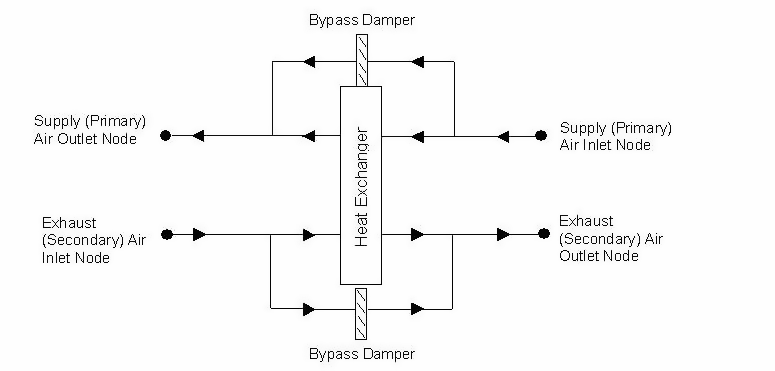
\includegraphics[width=0.9\textwidth, height=0.9\textheight, keepaspectratio=true]{media/image5455.png}
\caption{Schematic of the Sensible and Latent Air-to-Air Heat Exchanger \protect \label{fig:schematic-of-the-sensible-and-latent-air-to}}
\end{figure}

The sensible and latent air-to-air heat exchanger is typically used for exhaust or relief air heat recovery. Heat exchanger performance can be specified to transfer sensible energy, latent energy or both between the supply and exhaust air streams. The input requires no geometric data. Performance is defined by specifying sensible and/or latent effectiveness at 75\% and 100\% of the nominal (rated) supply air flow rate in both heating and cooling conditions (Table~\ref{table:operating-conditions-for-defining-heat}).

% table 74
\begin{longtable}[c]{p{3.0in}p{1.5in}p{1.5in}}
\caption{Operating Conditions for Defining Heat Exchanger Performance \label{table:operating-conditions-for-defining-heat}} \tabularnewline
\toprule 
Parameter & Conditions \tabularnewline
 & Heating & Cooling \tabularnewline
\midrule
\endfirsthead

\caption[]{Operating Conditions for Defining Heat Exchanger Performance} \tabularnewline
\toprule 
Parameter & Conditions \tabularnewline
 & Heating & Cooling \tabularnewline
\midrule
\endhead
Entering supply air temperature: \tabularnewline
Dry-bulb & 1.7°C (35°F) & 35°C (95°F) \tabularnewline
Wet-bulb & 0.6°C (33°F) & 26°C (78°F) \tabularnewline
Entering exhaust air temperature: \tabularnewline
Dry-bulb & 21°C (70°F) & 24°C (75°F) \tabularnewline
Wet-bulb & 14°C (58°F) & 17°C (63°F) \tabularnewline
\midrule
\multicolumn{3}{l}{Note: Conditions consistent with the Air-Conditioning and Refrigeration Institute’s}  \tabularnewline
\multicolumn{3}{l}{Standard 1060 (ARI 2001).} \tabularnewline
\bottomrule
\end{longtable}

Heat exchange between the supply and exhaust air streams occurs whenever the unit is scheduled to be available (availability schedule) and supply/exhaust air flows are present. This heat exchanger object can be used in conjunction with a conventional air-side economizer (i.e., specify an appropriate economizer control type in the Controller:OutdoorAir object), whereby heat exchange is suspended whenever the air-side economizer is active (i.e., air flow is fully bypassed around a fixed-plate heat exchanger or the rotation of a rotary heat exchanger is stopped). This object is also able to suspend heat exchange for the purpose of providing free cooling operation in the absence of a conventional air-side economizer (i.e., specify MinimumFlowWithBypass in the Controller:Outside Air object). Suspension of heat exchange during economizer mode may be customized as necessary using the economizer lockout field. Note that the Economizer Type must be set to something other than NoEconomizer for this control interaction to function.

\clearpage

Several methods of frost control are available to warm the heat exchanger core to prevent frost formation. Available methods are preheat, exhaust only, exhaust air recirculation, and minimum exhaust temperature. Preheat frost control uses a separate heater object placed in the supply inlet air stream to keep the air temperature above the frost threshold temperature. All other frost control methods are modeled within this heat exchanger object.

This heat exchanger object can also control the supply air outlet temperature to a setpoint when a setpoint manager and temperature schedule are used. This temperature control is accomplished through wheel speed modulation or bypassing supply air around the heat exchanger to maintain the desired setpoint and avoid overheating or overcooling the supply air.

\subsubsection{Model Description}\label{model-description-011}

The heat exchanger object models energy transfer between the supply air stream and the exhaust air stream according to the effectiveness values that are specified by the user in the input data file (see IO Reference Document, HeatExchanger:AirToAir:SensibleAndLatent). The operating volumetric air flow rate through the heat exchanger (i.e., the average of the actual supply and exhaust air flow rates for the simulation time step) should be between 50\% and 130\% of the nominal supply air flow rate specified for the heat exchanger. Operating air flow rates outside this range result in a warning message and a recommendation to adjust air flow rates to within the appropriate range.

The user must enter the sensible and latent effectiveness of the heat exchanger for heating and cooling conditions (Table~\ref{table:operating-conditions-for-defining-heat}) with balanced air flow (supply flow equal to the exhaust flow) at two flow rates: 75\% and 100\% of the nominal supply air flow rate. Heat exchanger manufacturers can typically provide this performance information, and it is also available for equipment contained in ARI's Certified Product Directory for Air-to-Air Energy Recovery Ventilation Equipment (ARI 2003). Values may be entered for sensible effectiveness, latent effectiveness, or both. The model assumes default values of 0.0 for sensible and latent effectiveness, thus requiring the user to input representative values for the heat exchanger being modeled.

To obtain the ``operating'' effectiveness of the heat exchanger at different air flow rates, the model first calculates the average volumetric air flow rate through the heat exchanger (average of the supply and exhaust air flow rates) for each simulation time step. Air flows through the heat exchanger may be unbalanced (supply greater than exhaust, or vice versa), but an unbalanced air flow ratio greater than 2:1 is not recommended~ (beyond this range a warning message is issued). The model determines the operating effectiveness of the heat exchanger by linear interpolation or extrapolation of the 100\% flow and 75\% flow effectiveness values specified in the input data file, using the average volumetric air flow rate through the heat exchanger. Extrapolation is allowed down to 50\% and up to 130\% of the nominal supply air flow rate (beyond this range a warning message is issued).

\begin{equation}
{\varepsilon_{operating,sensible}} = {\varepsilon_{sensible,75\%flow}} + ({\varepsilon_{sensible,100\%flow}} - {\varepsilon_{sensible,75\%flow}})\left( {\frac{{H{X_{flowratio}} - 0.75}}{{1 - 0.75}}} \right)
\label{eq:varepsilonoperatingsensible}
\end{equation}

\begin{equation}
{\varepsilon_{operating,latent}} = {\varepsilon_{latent,75\% \,flow}} + ({\varepsilon_{latent,100\% \,flow}} - {\varepsilon_{latent,75\% \,flow}})\left( {\frac{{H{X_{flowratio}} - 0.75}}{{1 - 0.75}}} \right)
\label{eq:varepsilonoperatinglatent}
\end{equation}

where:

\({\varepsilon_{operating,sensible}}\) is the operating sensible effectiveness of the heat exchanger

\({\varepsilon_{operating,latent}}\) is the operating latent effectiveness of the heat exchanger

\({\varepsilon_{sensible,75\% \,flow}}\) is the sensible effectiveness at 75\% airflow condition

\({\varepsilon_{sensible,100\% \,flow}}\) is the sensible effectiveness at 100\% airflow condition

\({\varepsilon_{latent,75\% \,flow}}\) is the latent effectiveness at 75\% airflow condition

\({\varepsilon_{latent,100\% \,flow}}\) is the latent effectiveness at 100\% airflow condition

\(H{X_{flowratio}}\) is the ratio of the average operating volumetric air flow rate {[}(supply flow plus exhaust flow) / 2.0{]} to the nominal supply air flow rate.

If the heat exchanger's supply air inlet temperature is less than the exhaust air inlet temperature, the operating sensible and latent effectivenesses are calculated using the 75\% and 100\% heating condition values; otherwise, the 75\% and 100\% cooling effectiveness values are used in Equations~\ref{eq:varepsilonoperatingsensible} and~\ref{eq:varepsilonoperatinglatent}.

The supply air conditions leaving the heat exchanger are determined using the heat exchanger operating effectiveness calculated above, the ratio of the air stream with the minimum heat capacity rate to the supply air stream heat capacity rate, and the difference in temperature or humidity ratio between the supply and exhaust inlet air:

\begin{equation}
{\dot{m} c_{p,min}} = MIN({\dot{m} c_{p,sup}},{\dot{m} c_{p,exh}})
\end{equation}

\begin{equation}
{T_{SupAirOut}} = {T_{SupAirIn}} + {\varepsilon_{operating,sensible}}\left( {\frac{\dot{m} c_{p,min}}{\dot{m} c_{p,sup}}} \right)({T_{ExhAirIn}} - {T_{SupAirIn}})
\end{equation}

\begin{equation}
{\omega_{SupAirOut}} = {\omega_{SupAirIn}} + {\varepsilon_{operating,latent}}\left( {\frac{{\mathop m\limits^ \bullet  cp,\min }}{{\mathop m\limits^ \bullet  cp,\sup }}} \right)({\omega_{ExhAirIn}} - {\omega_{SupAirIn}})
\end{equation}

where:

\({\dot{m} c_{p,min}}\) is the minimum heat capacity rate (W/K)

\({\dot{m} c_{p,sup}}\) is the heat capacity rate of the supply air stream (W/K)

\({\dot{m} c_{p,exh}}\) is the heat capacity rate of the exhaust air stream (W/K)

\emph{T\(_{SupAirOut}\)} is the supply air temperature leaving the heat exchanger (\(^{\circ}\)C)

\emph{T\(_{SupAirIn}\)} is the supply air inlet temperature (\(^{\circ}\)C)

\emph{T\(_{ExhAirIn}\)} is the exhaust air inlet temperature (\(^{\circ}\)C)

\({\omega_{SupAirOut}}\) is the supply air humidity ratio leaving the heat exchanger (kg/kg)

\({\omega_{SupAirIn}}\) is the supply air inlet humidity ratio (kg/kg)

\({\omega_{ExhAirIn}}\) is the exhaust air inlet humidity ratio (kg/kg).

Using the supply air outlet temperature and humidity ratio, the enthalpy of the supply air leaving the heat exchanger is calculated.

\begin{equation}
{h_{SupAirOut}} = PsyHFnTdbW({T_{SupAirOut}},{\omega_{SupAirOut}})
\end{equation}

where:

\emph{h\(_{SupAirOut}\)} is the enthalpy of the supply air leaving the heat exchanger (J/kg)

\emph{PsyHFnTdbW} is a psychrometric routine calculating air enthalpy as a function of temperature and humidity ratio.

If the predicted conditions of the supply air leaving the heat exchanger exceed the saturation curve (\textgreater{}100\% RH), then the temperature and humidity ratio of the air are reset to saturated conditions (= 100\% RH) at the enthalpy condition calculated above (\emph{h\(_{SupAirOut}\)).}

Next, the sensible and total heat recovery rates of the heat exchanger are calculated:

\begin{equation}
{\dot{Q}_{Sensible}} = \left( {\dot{m} c_{p,sup}} \right)({T_{SupAirIn}} - {T_{SupAirOut}})
\label{eq:QSensibleHX600}
\end{equation}

\begin{equation}
{\dot{Q}_{Total}} = {\dot{m}_{SupAir}}({h_{SupAirIn}} - {h_{SupAirOut}})
\label{eq:QTotalHX601}
\end{equation}

where:

\({\dot{Q}_{Sensible}}\) is the sensible heat recovery rate (W)

\({\dot{Q}_{Total}}\) is the total heat recovery rate (W)

\emph{h\(_{SupAirIn}\)} is the supply air inlet enthalpy (J/kg)

\({\dot{m}_{SupAir}}\) is the mass flow rate of the supply air stream (kg/s).

The conditions of the exhaust (secondary) air leaving the heat exchanger are then calculated:

\begin{equation}
{T_{ExhAirOut}} = {T_{ExhAirIn}} + \frac{\dot{Q}_{Sensible}}{\dot{m} c_{p,exh}}
\end{equation}

\begin{equation}
{h_{ExhAirOut}} = {h_{ExhAirIn}} + \frac{\dot{Q}_{Total}}{\dot{m}_{ExhAir}}
\end{equation}

\begin{equation}
{\omega_{ExhAirOut}} = PsyWFnTdbH({T_{ExhAirOut}},{h_{ExhAirOut}})
\end{equation}

\emph{where}:

\emph{T\(_{ExhAirOut}\)} is the exhaust air temperature leaving the heat exchanger (\(^{\circ}\)C)

\emph{h\(_{ExhAirOut}\)} is the exhaust air enthalpy leaving the heat exchanger (J/kg)

\({\dot{m}_{ExhAir}}\) is the mass flow rate of the exhaust air stream (kg/s)

\({\omega_{ExhAirOut}}\) is the exhaust air humidity ratio leaving the heat exchanger (kg/kg)

\emph{PsyWFnTdbH} is a psychrometric routine calculating air humidity ratio as a function of temperature and enthalpy.

As was done for the supply air, calculated exhaust air conditions beyond the saturation curve are reset to saturation conditions at the calculated air enthalpy value.

Once the air conditions leaving each side of the heat exchanger (supply and exhaust) are calculated, this air is blended with any bypass air that was directed around the heat exchanger core to determine the final air conditions leaving the heat exchanger unit. These outlet air conditions are used in Equations~\ref{eq:QSensibleHX600} and~\ref{eq:QTotalHX601} to determine the sensible and total heat recovery rate for the overall heat exchanger unit. The latent heat recovery rate for the overall unit is then calculated as the difference between the total and sensible heat recovery rates:

\begin{equation}
{\dot{Q}_{Latent}} = {\dot{Q}_{Total}} - {\dot{Q}_{Sensible}}
\end{equation}

Heat recovery electric power is the electric consumption rate of the unit in watts. The nominal electric power rate for the heat exchanger is specified in the input data file, and can be used to model controls (transformers, relays, etc.) and/or a motor for a rotary heat exchanger. The model assumes that this electric power is consumed whenever the heat exchanger is scheduled to operate and supply/exhaust air flow rates exist. The electric power is assumed to be zero for all other times or if heat exchange is suspended to provide free cooling (economizer operation). None of this electric power is assumed to contribute thermal load to either of the heat exchanger air streams.

At the end of each HVAC simulation time step, this object reports the sensible, latent and total heat recovery rates for the overall unit as calculated above. The heat recovery rates are reported separately for times when the supply air is heated and when it is cooled (Ref: HeatExchanger:AirToAir:SensibleAndLatent in the EnergyPlus Input Output Reference). The heat recovery electric power is also reported for each simulation time step. In addition to the heat recovery rates and electric power, heating/cooling energy transferred to the supply air and the electric energy consumption by the heat exchanger unit are calculated for the time step being reported as follows:

\begin{equation}
{Q_{SensibleCooling}} = {\dot{Q}_{SensibleCooling}} * TimeStepSys * 3600
\end{equation}

\begin{equation}
{Q_{LatentCooling}} = {\dot{Q}_{LatentCooling}} * TimeStepSys * 3600
\end{equation}

\begin{equation}
{Q_{TotalCooling}} = {\dot{Q}_{TotalCooling}} * TimeStepSys * 3600
\end{equation}

\begin{equation}
{Q_{SensibleHeating}} = {\dot{Q}_{SensibleHeating}} * TimeStepSys * 3600
\end{equation}

\begin{equation}
{Q_{LatentHeating}} = {\dot{Q}_{LatentHeating}} * TimeStepSys * 3600
\end{equation}

\begin{equation}
{Q_{TotalHeating}} = {\dot{Q}_{TotalHeating}} * TimeStepSys * 3600
\end{equation}

\begin{equation}
{E_{HXUnit}} = {P_{HXUnit}} * TimeStepSys * 3600
\end{equation}

where: 

\(Q_{SensibleCooling}\) is the output variable `Heat Exchanger Sensible Cooling Energy, J'

\({\dot{Q}_{SensibleCooling}}\) is the output variable `Heat Exchanger Sensible Cooling Rate, W' which is equal to \({\dot{Q}_{Sensible}}\) during times when the supply air is cooled

\emph{TimeStepSys} is the HVAC system simulation time step, hr

\(Q_{LatentCooling}\) is the output variable `Heat Exchanger Latent Cooling Energy, J'

\({\dot{Q}_{LatentCooling}}\) is the output variable `Heat Exchanger Latent Cooling Rate, W' which is equal to \({\dot{Q}_{Latent}}\) during times when the supply air is dehumidified

\(Q_{TotalCooling}\) is the output variable `Heat Exchanger Total Cooling Energy, J'

\({\dot{Q}_{TotalCooling}}\) is the output variable `Heat Exchanger Total Cooling Rate, W' which is equal to \({\dot{Q}_{Total}}\) during times when the supply air enthalpy is reduced

\(Q_{SensibleHeating}\) is the output variable `Heat Exchanger Sensible Heating Energy, J'

\({\dot{Q}_{SensibleHeating}}\) is the output variable `Heat Exchanger Sensible Heating Rate, W' which is equal to \({\dot{Q}_{Sensible}}\) during times when the supply air is heated

\(Q_{LatentHeating}\) is the output variable `Heat Exchanger Latent Heating Energy, J' and also the output variable `Heat Exchanger Latent Gain Energy, J'

\({\dot{Q}_{LatentHeating}}\) is the output variable `Heat Exchanger Latent Gain Rate, W' which is equal to \({\dot{Q}_{Latent}}\) during times when the supply air is humidified

\(Q_{TotalHeating}\) is the output variable `Heat Exchanger Total Heating Energy, J'

\({\dot{Q}_{TotalHeating}}\) is the output variable `Heat Exchanger Total Heating Rate, W' which is equal to \({\dot{Q}_{Total}}\) during times when the supply air enthalpy is increased

\({E_{HXUnit}}\) is the output variable `Heat Exchanger Electric Energy, J'

\({P_{HXUnit}}\) is the output variable `Heat Exchanger Electric Power, W'.

\subsubsection{Frost Control Methods}\label{frost-control-methods}

In cold weather, frost can form on the heat exchanger causing a reduction in air flow and heat recovery performance. Various strategies can be employed to limit frost formation. Heat exchangers that transfer total energy (sensible plus latent) usually have a lower frost threshold temperature than sensible-only heat exchangers. Frost threshold temperatures for sensible-only heat exchangers may be -1\(^{\circ}\)C to -12\(^{\circ}\)C for plate and rotary heat exchangers respectively, while those for comparable total (sensible plus latent) heat exchangers may be 10\(^{\circ}\)C lower. The frost threshold temperature for a specific application is dependent on the exhaust air dry-bulb temperature and relative humidity, heat exchanger type (e.g., sensible-only or total heat exchange, flat plate or rotary), and the heat exchanger effectiveness. Consult manufacturer's literature to obtain specific frost threshold temperatures for the heat exchanger being modeled.

Four frost control strategies can be modeled for this air-to-air heat exchanger unit. Each of these four strategies is discussed in detail below.

\subsubsection{Preheat}\label{preheat}

One method to control frost formation is to preheat the cold outdoor (supply) air entering the heat exchanger. When a preheat coil is used for frost control, a separate heating coil object must be placed in the supply air stream at the inlet to the heat exchanger (Coil:Heating:Water, Coil:Heating:Electric or Coil:Heating:Fuel). The preheat coil should be controlled to maintain a minimum supply air inlet temperature thereby eliminating frost buildup on the heat exchanger core. When modeling preheat frost control, specify ``None'' as the frost control method in the heat exchanger object. When modeling this heat exchanger as part of an air loop, refer to the objects AirLoopHVAC:OutdoorAirSystem and SetpointManager:Scheduled the EnergyPlus Input Output Reference for additional information on specifying a preheat coil and controlling its supply air temperature.This frost control method is not currently available when this heat exchanger is being used as part of the compound object ZoneHVAC:EnergyRecoveryVentilator.

\subsubsection{Exhaust Only}\label{exhaust-only}

This method of frost control bypasses the incoming supply air around the heat exchanger core thereby warming the core using the exiting exhaust air. This method is similar to `supply air off' frost control where the supply air fan is turned off for a predetermined period of time while the exhaust air fan continues to operate. For the `supply air off' method, the supply air flow is stopped for a period of time thereby reducing the ventilation air supplied to the zone(s). In addition, the building may be negatively pressurized for the period of time that the supply air flow is stopped since the exhaust air fan continues to operate. On the other hand, the `exhaust only' method of frost control modeled by EnergyPlus continues to provide outdoor ventilation air to the zone(s), but this air is simply bypassed around the heat exchanger core for a portion of the time and the potential problem with negatively pressurizing the building is avoided. Since the supply airflow rate through the heat exchanger core is purposely reduced to control frost formation, average volumetric airflow rates below 50\% of nominal are allowed when this frost control is active and no warning message is issued.

The user enters a threshold temperature, an initial defrost time fraction, and a rate of defrost time fraction increase. When the temperature of the supply air (e.g., outdoor air) entering the heat exchanger is equal to or below the specified threshold temperature, the fractional amount of time that the supply air is bypassed around the heat exchanger core is determined from the following equation:

\begin{equation}
{X_{DefrostTime}} = {X_{Initial}} + {X_{RateofIncrease}}({T_{Threshold}} - {T_{SupAirIn}})
\end{equation}

where:

\({X_{DefrostTime}}\) is the fractional time period for frost control \(\left( {0 \leq {X_{DefrostTime}} \leq 1} \right)\)

\({X_{Initial}}\) is the initial defrost time fraction

\({X_{RateofIncrease}}\) is the rate of defrost time fraction increase (K\(^{-1}\))

\({T_{Threshold}}\) is the threshold temperature (\(^{\circ}\)C)

\({T_{SupAirIn}}\) is the supply air inlet temperature (\(^{\circ}\)C).

During the defrost time, supply air flow is fully bypassed around the heat exchanger core and no heat transfer takes place. For the remainder of the time period, no air is bypassed and full heat exchange is achieved. The average supply air flow bypassed around the heat exchanger core is calculated as follows:

\begin{equation}
{\dot{m}_{SupAirBypass}} = ({X_{DefrostTime}}){\dot{m}_{SupAir}}
\end{equation}

To determine the average heat transfer rates for the simulation time step, the supply air outlet conditions are first calculated as if the heat exchanger were not in defrost mode (see previous section, Model Description). The sensible and total heat transfer rates are then calculated and multiplied by the fractional time period that the heat exchanger is \emph{not} in defrost mode (1-\emph{X\(_{DefrostTime}\)}).

\begin{equation}
{\dot{Q}_{Sensible}} = (1 - {X_{DefrostTime}})\left( {\dot{m} c_{p,sup}} \right)({T_{SupAirIn}} - {T_{SupAirOut}})
\end{equation}

\begin{equation}
{\dot{Q}_{Total}} = (1 - {X_{DefrostTime}}){\dot{m}_{SupAir}}({h_{SupAirIn}} - {h_{SupAirOut}})
\end{equation}

Once the average heat transfer rates are determined, the average conditions of the supply air exiting the overall heat exchanger unit are calculated as follows:

\begin{equation}
{T_{SupAirOut}} = {T_{SupAirIn}} - \frac{\dot{Q}_{Sensible}}{\dot{m} c_{p,sup}}
\end{equation}

\begin{equation}
{h_{SupAirOut}} = {h_{SupAirIn}} - \frac{\dot{Q}_{Total}}{\dot{m}_{SupAir}}
\end{equation}

\begin{equation}
{\omega_{SupAirOut}} = PsyWFnTdbH({T_{SupAirOut}},{h_{SupAirOut}})
\end{equation}

As described previously, if the predicted conditions of the exiting supply air exceed the saturation curve (\textgreater{}100\% RH), then the temperature and humidity ratio of the air are reset to saturated conditions ( = 100\% RH) at the enthalpy condition calculated above (\emph{h\(_{SupAirOut}\))}. If the supply air temperature is reset, the average sensible heat transfer rate is recalculated before the exhaust air outlet conditions are determined:

\begin{equation}
{T_{ExhAirOut}} = {T_{ExhAirIn}} + \frac{\dot{Q}_{Sensible}}{\dot{m} c_{p,exh}}
\end{equation}

\begin{equation}
{h_{ExhAirOut}} = {h_{ExhAirIn}} + \frac{\dot{Q}_{Total}}{\dot{m}_{ExhAir}}
\end{equation}

\begin{equation}
{\omega_{ExhAirOut}} = PsyWFnTdbH({T_{ExhAirOut}},{h_{ExhAirOut}})
\end{equation}

\subsubsection{Exhaust Air Recirculation}\label{exhaust-air-recirculation}

This method of frost control routes exhaust (outlet) air back through the supply side of the heat exchanger to warm the core. Since this method routes exhaust air back into the building, the building is typically not depressurized when this frost control is active. However, the incoming supply (outdoor ventilation) air flow is stopped for the fractional period of time that frost control is active. If significant periods of time exist when outdoor temperatures are below the selected threshold temperature and outdoor ventilation air is continuously required, an alternative method of frost control should be considered.

The user enters a threshold temperature, an initial defrost time fraction, and a rate of defrost time fraction increase. When the temperature of the inlet supply air (e.g., outdoor air) is equal to or below the specified threshold temperature, the fractional amount of time that this heat exchanger frost control strategy is active is determined from the following equation:

\begin{equation}
{X_{DefrostTime}} = {X_{Initial}} + {X_{RateofIncrease}}({T_{Threshold}} - {T_{SupAirIn}})
\end{equation}

The air mass flow rate of the supply air leaving the heat exchanger unit is then calculated using the defrost time fraction calculated above the mass flow rates of supply and exhaust air entering the unit.

\begin{equation}
{\dot{m}_{SupAirOut}} = (1 - {X_{DefrostTime}}){\dot{m}_{SupAirIn}} + {X_{DefrostTime}}{\dot{m}_{ExhAirIn}}
\end{equation}

The model assumes that no heat exchange occurs during defrost, and the average supply supply air conditions are simply a blend of the conditions when the unit is \emph{not} in defrost and the exhaust air inlet conditions during defrost operation:

\begin{equation}
{T_{SupAirOut}} = \frac{{(1 - {X_{DefrostTime}}){{\dot{m}_{SupAirIn}}}{T_{SupAirOut,NoDefrost}} + {X_{DefrostTime}}{{\dot{m}_{ExhAirIn}}}{T_{ExhAirIn}}}}{{{{\dot{m}_{SupAirOut}}}}}
\end{equation}

\begin{equation}
{\omega_{SupAirOut}} = \frac{{(1 - {X_{DefrostTime}}){{\dot{m}_{SupAirIn}}}{\omega_{SupAirOut,NoDefrost}} + {X_{DefrostTime}}{{\dot{m}_{ExhAirIn}}}{\omega_{ExhAirIn}}}}{{{{\dot{m}_{SupAirOut}}}}}
\end{equation}

\begin{equation}
{h_{SupAirOut}} = PsyHFnTdbW({T_{SupAirOut}},{\omega_{SupAirOut}})
\end{equation}

The operating effectivenesses of the heat exchanger are initially calculated according to Equations~\ref{eq:varepsilonoperatingsensible} and~\ref{eq:varepsilonoperatinglatent} assuming no defrost operation. Since the supply air flow across the heat exchanger core is not reduced during defrost operation, the sensible and latent effectiveness are therefore derated (for reporting purposes) in direct proportion to the fraction of time that frost control is \emph{not} active.

\begin{equation}
{\varepsilon_{operating,sensible}} = (1 - {X_{DefrostTime}}){\varepsilon_{operating,sensible}}
\end{equation}

\begin{equation}
{\varepsilon_{operating,latent}} = (1 - {X_{DefrostTime}}){\varepsilon_{operating,latent}}
\end{equation}

Since the exhaust outlet air is recirculated through the supply side of the heat exchanger core, the incoming supply air and exiting exhaust air flows are stopped for the fraction of the time when frost control is active. The average air mass flow rate at the supply air inlet and the exhaust air outlet nodes are therefore reduced accordingly.

\begin{equation}
{\dot{m}_{SupAirIn}} = (1 - {X_{DefrostTime}}){\dot{m}_{SupAirIn}}
\end{equation}

\begin{equation}
{\dot{m}_{ExhAirOut}} = (1 - {X_{DefrostTime}}){\dot{m}_{ExhAirOut}}
\end{equation}

The conditions of the exiting (outlet) exhaust air (temperature, humidity ratio and enthalpy) are reported as the values when frost control is \emph{not} active (i.e., the conditions when exhaust air is actually leaving the unit).

\subsubsection{Minimum Exhaust Temperature}\label{minimum-exhaust-temperature}

With this frost control method, frost formation is avoided by continuously maintaining the temperature of the exhaust air leaving the heat exchanger core above a specified setpoint. The minimum exhaust air temperature is maintained by modulating heat exchanger rotational speed or by bypassing supply air around a plate heat exchanger. For this frost control method, the user must only enter the threshold (minimum) temperature.

For the case of modulating heat exchanger rotation, the operating effectivenesses and outlet air conditions are first calculated as if the heat exchanger is \emph{not} in defrost mode (see Model Description). If the resulting temperature of the exhaust air leaving the heat exchanger core is below the specified threshold temperature, then the operating effectivenesses are reduced as follows:

\begin{equation}
{X_{DefrostTime}} = \frac{{({T_{Threshold}} - {T_{ExhAirOut}})}}{{({T_{ExhAirIn}} - {T_{ExhAirOut}})}}
\end{equation}

\begin{equation}
{\varepsilon_{operating,sensible}} = (1 - {X_{DefrostTime}}){\varepsilon_{operating,sensible}}
\end{equation}

\begin{equation}
{\varepsilon_{operating,latent}} = (1 - {X_{DefrostTime}}){\varepsilon_{operating,latent}}
\end{equation}

The supply air and exhaust air outlet conditions are then recalculated using these reduced effectiveness values. Finally the sensible, latent and total heat recovery rates are calculated along with the unit's electric power and electric consumption.

The calculation procedure is slightly different for the case of a plate heat exchanger where the supply air is bypassed around the heat exchanger core. Since the volumetric air flow rate through the heat exchanger core is reduced when frost control is active, an iterative process is used to determine the operating effectiveness of the heat exchanger. The operating effectivenesses and outlet air conditions are first calculated as if the heat exchanger is \emph{not} in defrost mode (see Model Description). If the resulting temperature of the exhaust air leaving the heat exchanger core is below the specified threshold temperature, then the fractional defrost time is calculated as follows:

\begin{equation}
{X_{DefrostTime}} = \frac{{({T_{Threshold}} - {T_{ExhAirOut}})}}{{({T_{ExhAirIn}} - {T_{ExhAirOut}})}}
\end{equation}

The iteration process then begins to determine the heat exchanger effectiveness and the exhaust air outlet temperature as if frost control were active. The operating mass flow rate through the supply side of the heat exchanger core is calculated.

\emph{Beginning of iteration process:}

\begin{equation}
{\dot{m}_{SupAirCore}} = (1 - {X_{DefrostTime}}){\dot{m}_{SupAirIn}}
\end{equation}

\begin{equation}
{\dot{m}_{SupAirBypass}} = ({X_{DefrostTime}}){\dot{m}_{SupAirIn}}
\end{equation}

The ratio of average volumetric flow rate through the heat exchanger core to heat exchanger's nominal volumetric flow rate (\emph{HX\(_{flowratio}\)}) is then determined and used to calculate the operating effectiveness of the heat exchanger using Equations~\ref{eq:varepsilonoperatingsensible} and~\ref{eq:varepsilonoperatinglatent}. Since the supply airflow rate through the heat exchanger core is purposely reduced to control frost formation, average volumetric airflow rates below 50\% of nominal are allowed and no warning message is issued. Supply air outlet temperature (leaving the heat exchanger core), sensible heat transfer, and exhaust air outlet temperature are then calculated using the revised heat exchanger effectiveness.

\begin{equation}
{T_{SupAirOut}} = {T_{SupAirIn}} + {\varepsilon_{operating,sensible}}\left( {\frac{{\dot{m}  c_{p,min}}}{{\dot{m} c_{p,sup}}}} \right)({T_{ExhAirIn}} - {T_{SupAirIn}})
\end{equation}

\begin{equation}
{\dot{Q}_{Sensible}} = (1 - {X_{DefrostTime}})\left( {\dot{m} c_{p,sup}} \right)({T_{SupAirInlet}} - {T_{SupAirOutlet}})
\end{equation}

\begin{equation}
{T_{ExhAirOut}} = {T_{ExhAirIn}} + \frac{\dot{Q}_{Sensible}}{\dot{m} c_{p,exh}}
\end{equation}

The error between the exhaust outlet temperature and the threshold temperature for frost control and a new defrost time fraction are subsequently calculated.

\begin{equation}
Error = {T_{ExhAirOut}} - {T_{Threshold}}
\end{equation}

\begin{equation}
{X_{DefrostTime}} = {X_{DefrostTime}}\,\left( {\frac{{{T_{ExhAirIn}} - {T_{ExhAirOut}}}}{{{T_{ExhAirIn}} - {T_{Threshold}}}}} \right)
\end{equation}

\emph{End of iteration process:}

The iteration process ends when the calculated error is within an error tolerance of 0.001.~ The air streams passing through the heat exchanger core and bypassing the core through the bypass damper are then blended together to provide the air conditions leaving the heat exchanger unit. Finally the sensible, latent and total heat recovery rates are calculated along with the unit's electric power and electric consumption.

\subsubsection{Economizer Operation}\label{economizer-operation}

A conventional air-side economizer may be used in conjunction with this heat exchanger object. The air-side economizer is specified through the use of an outside air controller (see object: Controller:OutdoorAir). Specify the appropriate economizer control type, and provide the required control points and air flow rates as defined in the outside air controller object. Energy transfer provided by the heat exchanger will be suspended whenever free cooling is available (i.e., when the air-side economizer is activated) and \emph{the user specified economizer lockout input is specified as Yes}. For plate heat exchangers, heat transfer is suspended by fully bypassing the supply and exhaust air around the heat exchanger core. For rotary heat exchangers, air flows continue through the core but it is assumed that heat exchanger rotation is stopped.

Heat exchange can also be suspended for the purposes of providing free cooling operation in the absence of a conventional air-side economizer. In this case specify ``MinimumFlowWithBypass'' as the economizer choice and again provide the required control points as defined in the outside air controller object. Energy transfer provided by the heat exchanger will be suspended whenever free cooling is available and \emph{the user specified economizer lockout input is specified as Yes}, however the supply air flow rate will remain at the minimum value specified in the outside air controller object. Note that the Economizer Type must be set to something other than NoEconomizer for this control interaction to function.

If economizer operation is not required, specify ``NoEconomizer'' as the economizer control type in the outside air controller object. The heat exchanger will operate according to its availability schedule and free cooling will not be provided. . If economizer operation \emph{is} required and the heat exchanger \emph{should not} provide free cooling, specify the input for the heat exchanger's economizer lockout as No and heat recovery will remain active during economizer mode.

Heat recovery for this heat exchanger may also be suspended during a high humidity control event (see object Controller:OutdoorAir) in a similar manner. Specifying Yes for economizer lockout will also suspend heat recovery when high humidity control is activated. The default value for economizer lockout is Yes and must be specifically entered as No to disable the economizer or high humidity control lockout feature.

\subsubsection{Supply Air Outlet Temperature Control}\label{supply-air-outlet-temperature-control}

This heat exchanger object can also control the supply air outlet temperature to a setpoint to avoid overheating or overcooling the supply air. This temperature control is accomplished through wheel speed modulation or bypassing supply air around the heat exchanger. To model this temperature control, the user must specify `Yes' for the Supply Air Outlet Temperature Control field in this heat exchanger object, and a separate setpoint manager (see object: SetpointManager:Scheduled) and temperature schedule must be specified for the heat exchanger unit's supply air outlet node.

This control strategy is typically used in conjunction with economizer operation (see object Controller:OutdoorAir), and an example control profile is shown in the figure below. When the outdoor air temperature falls to the specified maximum limit for economizer operation, heat exchange is suspended (air is fully bypassed around the heat exchanger core or heat exchanger rotation is stopped). The figure below shows economizer operation being initiated based on outdoor temperature but other triggers can be used (e.g.~differential temperature {[}outdoor temperature with respect to exhaust air temperature{]}, single point enthalpy or differential enthalpy). Heat exchange remains suspended until the outdoor temperature falls to the minimum temperature (temperature lower limit) for economizer control. The setpoint for the supply air outlet temperature control should match the economizer temperature lower limit.

As the outdoor air temperature falls further below the setpoint for the supply air outlet temperature (same as the economizer lower temperature limit), the heat exchanger bypass dampers will modulate closed to maintain the desired supply air temperature for a plate heat exchanger. For a rotary heat exchanger the rotary heat exchanger speed will gradually increase to maintain the desired supply air temperature. Modulation of heat exchanger performance will continue until the supply air temperature setpoint can no longer be maintained. This control will attempt to achieve the desired temperature set point whether the heat exchanger is cooling or heating the supply air stream. Care should be used to set the supply outlet air temperature set point to the desired value for proper control.

\begin{figure}[hbtp] % fig 251
\centering

\includegraphics[width=0.9\textwidth, height=0.9\textheight, keepaspectratio=true]{media/image5550.png}
\caption{Air to Air Heat Exchanger with Supply Air Temperature Control \protect \label{fig:air-to-air-heat-exchanger-with-supply-air}}
\end{figure}

Other types of temperature setpoint control may also be used. For example, the operation described here is used to minimize heating energy and proper control of the supply air temperature set point could also be used to minimize cooling energy or minimize both heating and cooling energy.

\subsubsection{References}\label{references-027}

ARI. 2001. Rating Air-to-Air Heat Exchangers for Energy Recovery Ventilation Equipment. Arlington, Virginia: Air-Conditioning \& Refrigeration Institute.

ARI. 2003. Certified Product Directory for Air-to-Air Energy Recovery Ventilation Equipment. Arlington, Virginia: Air-Conditioning \& Refrigeration Institute.

\subsection{Air System Air-To-Air Flat Plate Heat Exchanger}\label{air-system-air-to-air-flat-plate-heat-exchanger}

\subsubsection{Overview}\label{overview-1-007}

The input object HeatExchanger:AirToAir:FlatPlate provides an NTU -- effectiveness model of a static flat plate air-to-air heat exchanger. Humidity issues are ignored in this model. A full, detailed description of the model can be found in the reference.

The inputs for the model are the design values for the primary air flow rate, primary air inlet and outlet temperature,~ secondary air flow rate, and secondary air inlet temperature. No design UAs are required: instead, the ratio (at design conditions) of the primary \emph{hA} to the secondary \emph{hA} (\emph{r\(_{hA}\)}) is input. The flow configuration is also an input (counter, parallel, or crossflow).

An important feature of this model is that the heat exchanger total \emph{UA} is a time varying function of the primary and secondary mass flow rates and inlet temperatures.

\subsubsection{Model Description}\label{model-description-1-007}

The design inlet / outlet conditions determine a design effectiveness \emph{eff}\(_{des}\). From the design capacity flow ratio, the flow arrangement, and \emph{eff}\(_{des}\), the NTU -- effectiveness formulas give the \emph{NTU\(_{des}\)} and \emph{UA\(_{des}\)}.

The time varying calculations proceed as follows. First, the \emph{UA} is determined:

\begin{equation}
UA = U{A_{des}}({r_{hA}} + 1)/({({\dot m_{p,des}}{T_{p,des}}/{\dot m_p}{T_p})^{.78}} + {r_{hA}}{({\dot m_{s,des}}{T_{s,des}}/{\dot m_s}{T_s})^{.78}})
\end{equation}

where \emph{des} means \emph{design}, \emph{p} means \emph{primary}, \emph{s} means \emph{secondary}, \emph{T} is air stream temperature, and \(\dot m\) is air stream mass flow rate. From the \emph{UA} and the capacity flow ratio the \emph{NTU} is determined: \(NTU = UA/{C_{\min }}\). Then the NTU -- effectiveness formulas are used to calculate the effectiveness. From the effectiveness and the inlet conditions, outlet condtions are determined.

\subsubsection{Economizer Operation}\label{economizer-operation-1}

A conventional air-side economizer may be used in conjunction with this heat exchanger object. The air-side economizer is specified through the use of an outside air controller (see object: Controller:OutdoorAir). Specify the appropriate economizer control type, and provide the required control points and air flow rates as defined in the outside air controller object. Energy transfer provided by the heat exchanger will be suspended whenever free cooling is available (i.e., when the air-side economizer is activated) or high humidity control is active and \emph{the user specified economizer lockout input is specified as Yes}. For this flat plate heat exchanger, heat transfer is suspended by fully bypassing the supply and exhaust air around the heat exchanger core. If the economizer lockout is specified as No, the flat plate heat exchanger is operational even when economizer or high humidity mode is active. The default value for economizer lockout is Yes and must be specifically entered as No to disable the economizer or high humidity control lockout feature.

\subsubsection{References}\label{references-1-010}

M. Wetter. 1999. \emph{Simulation Model: Air-To-Air Plate Heat Exchanger}, LBNL-42354. This document can be downloaded from \href{http://simulationresearch.lbl.gov}{\emph{http://simulationresearch.lbl.gov}}.

\subsection{Air System Air-To-Air Balanced Flow Desiccant Heat Exchanger}\label{air-system-air-to-air-balanced-flow-desiccant-heat-exchanger}

\subsubsection{Overview}\label{overview-2-006}

The input object HeatExchanger:Desiccant:BalancedFlow provides a model for a desiccant heat exchanger that is an HVAC component used to model both temperature (sensible) and moisture (latent) heat exchange between two air streams (Figure~\ref{fig:schematic-of-the-balanced-flow-desiccant-heat}). The model assumes balanced air flow through the regeneration and process sides of the heat exchanger (i.e., regeneration and process air volume flow rates and face velocities are the same). Heat exchanger performance is specified through a performance data type object (e.g., Heat Exchanger:Desiccant:BalancedFlow:Performance Data Type 1). Refer to the EnergyPlus Input Output Reference for the specific input syntax for this desiccant heat exchanger object.

\begin{figure}[hbtp] % fig 252
\centering

\includegraphics[width=0.9\textwidth, height=0.9\textheight, keepaspectratio=true]{media/image5554.png}
\caption{Schematic of the Balanced Flow Desiccant Heat Exchanger \protect \label{fig:schematic-of-the-balanced-flow-desiccant-heat}}
\end{figure}

EnergyPlus has another air-to-air heat exchanger object for modeling sensible and latent heat transfer between two air streams that uses the input object HeatExchanger:AirToAir:SensibleAndLatent. That heat exchanger model uses effectiveness values specified by the user to determine exiting air conditions from each side of the heat exchanger. In contrast, the balanced flow desiccant heat exchanger references a performance data type object (e.g., HeatExchanger:Desiccant:BalancedFlow:PerformanceDataType1) which defines the model equations, user-specified model coefficients, and min/max limits for the model's independent and dependent variables.

\subsubsection{Model Description}\label{model-description-2-006}

This heat exchanger is a simple object that performs three basic functions:

\begin{enumerate}
\item Informs the associated performance data type object (e.g., HeatExchanger:Desiccant:Balanc-edFlow:PerformanceDataType1) if it should calculate heat exchange for a simulation time step, or if heat exchange is suspended for the time step (i.e., bypass air flow around a fixed-plate heat exchanger or stop the rotation of a rotary heat exchanger),
\item Passes the process and regeneration air inlet conditions (e.g., dry-bulb temperature, humidity ratio, air mass flow rate) to the associated performance data type object, and
\item Reports the total, sensible and latent cooling/heating rates and electric power based on the results from the performance data type model that is specified.
\end{enumerate}

While the desiccant heat exchanger object's availability to provide heat exchange between the two air streams is determined by the user-specified availability schedule, other objects that call this heat exchanger object can also control its heat exchange during a simulation time step. Currently, this desiccant heat exchanger model can be referenced by two compound objects: CoilSystem:Cooling:DX:HeatExchangerAssisted and Dehumidifier:Desiccant:System, both of which are used to provide enhanced dehumidification over conventional systems. If this heat exchanger is referenced by a compound object, the compound object will control heat exchanger operation (i.e., tell the heat exchanger if heat exchange is needed or not for each simulation time step). Details for how the compound objects control exchanger operation are described elsewhere in this document (ref. CoilSystem:Cooling:DX:HeatExchangerAssisted and Dehumidifier:Desiccant:System).

This desiccant heat exchanger object may also be specified directly in a AirLoopHVAC (air loop BranchList) or in an AirLoopHVAC:OutdoorAirSystem:EquipmentList without being referenced by a compound object. If specified directly in a AirLoopHVAC loop or AirLoopHVAC:OutdoorAirSystem:EquipmentList, then the heat exchanger can be controlled to provide heat exchange based on a maximum and/or minimum humidity setpoint placed on the process air outlet node (ref. SetpointManagers). If no humidity setpoints are provided on this node, then heat exchange will be provided whenever the heat exchanger is available to operate (via its availability schedule) and there is a temperature and/or humidity ratio difference between the two air streams. Further details regarding heat exchanger control via humidity setpoints on the process air outlet node are described in the section for the associated data type object (e.g., HeatExchanger:Desiccant:BalancedFlow:PerformanceDataType1).

The balanced flow desiccant heat exchanger model first checks for three conditions to be true before calling the specified performance data type model to calculate heat exchanger performance:

\begin{itemize}
\item Non-zero air mass flow rates on the process and regeneration inlet air nodes,
\item Desiccant heat exchanger is available to operate based on its availability schedule,
\item If a compound object is calling this desiccant heat exchanger, it is requesting that heat exchange be provided.
\end{itemize}

If any of these conditions is false, then heat exchange is suspended and the model simply passes the air conditions on the process and regeneration air inlet nodes to the respective outlet air nodes. In addition, the heat exchanger electric power is set to zero.

If all of the above conditions are true, then heat exchange is active and the specified performance data type model is called to calculate the process and regeneration outlet air conditions and heat exchanger electric power. Immediately before this call to the performance data type model, a check is made to determine if the operating air flow rates through the heat exchanger (i.e., the actual air flow rates for the simulation time step) are equal (balanced flow). If a difference of more than 2\% exists between the process and regeneration air flow rates at any time during the simulation, a warning is issued.

After the specified performance data type model calculates the process/regeneration air outlet conditions and heat exchanger electric power, the balanced flow desiccant heat exchanger model uses that information to report overall performance. Specifically, the heat exchanger's sensible, latent and total heating and cooling rates are calculated for the process air side of the heat exchanger. Since energy must be conserved, the same heating or cooling rates apply to the regeneration air stream although they are opposite in heat transfer direction (e.g., a sensible cooling rate on the process air side of the heat exchanger would indicate an equivalent sensible heating rate on the regeneration air side).

\begin{equation}
{\dot{Q}_{Sensible}} = {\dot{m}_{Proc}} {C_{p_{Proc,in}}} \left( {{T_{Proc,out}} - {T_{Proc,in}}} \right)
\end{equation}

\begin{equation}
{\dot{Q}_{Total}} = {\dot{m}_{Proc}}\left( {{h_{Proc,out}}\, - \,{h_{Proc,in}}} \right)
\end{equation}

\begin{equation}
{\dot{Q}_{Latent}} = {\dot{Q}_{Total}} - {\dot{Q}_{Sensible}}
\end{equation}

where:

\({\dot{Q}_{Sensible}}\) is the sensible heat transfer rate to the process air stream (W)

\({\dot{Q}_{Total}}\) is the total heat transfer rate to the process air stream (W)

\({\dot{Q}_{Latent}}\) is the latent heat transfer rate to the process air stream (W)

\({\dot{m}_{Proc}}\) is the process air mass flow rate (kg/s)

\({C_{p_{Proc,in}}}\) is the specific heat of inlet process air (J/kg-K)

\({T_{Proc,out}}\) is the process air outlet temperature (°C)

\({T_{Proc,in}}\) is the process air inlet temperature (°C)

\({h_{Proc,out}}\) is the process air outlet enthalpy (J/kg)

\({h_{Proc,in}}\) is the process air inlet enthalpy (J/kg).

To simplify the accounting of heat exchanger performance, the sensible, latent, and total heat transfer rates for the process side of the heat exchanger are stored in cooling and heating report variables. For example, if the sensible heat transfer rate is negative, the absolute value is stored in a ``cooling'' rate report variable. Conversely, if the sensible heat transfer rate is positive, the value is stored in a ``heating'' rate report variable. Similar accounting is performed for the latent and total heat transfer rate variables as follows:

\begin{equation}
IF \left( {{{\dot{Q}_{Sensible}}} \leq 0} \right) {\dot{Q}_{SensibleCooling}} = ABS\left( {\dot{Q}_{Sensible}} \right)
\end{equation}

\begin{equation}
IF \left( {{\dot{Q}_{Sensible}} > 0} \right){\dot{Q}_{SensibleHeating}} = {\dot{Q}_{Sensible}}
\end{equation}

\begin{equation}
IF \left( {{{\dot{Q}_{Latent}}} \leq 0} \right) {\dot{Q}_{LatentCooling}} = ABS\left( {\dot{Q}_{Latent}} \right)
\end{equation}

\begin{equation}
IF \left( {{\dot{Q}_{Latent}} > 0} \right){\dot{Q}_{LatentHeating}} = {\dot{Q}_{Latent}}
\end{equation}

\begin{equation}
IF \left( {{{\dot{Q}_{Total}}} \leq 0} \right) {\dot{Q}_{TotalCooling}} = ABS\left( {\dot{Q}_{Total}} \right)
\end{equation}

\begin{equation}
IF \left( {{\dot{Q}_{Total}} > 0} \right){\dot{Q}_{TotalHeating}} = {\dot{Q}_{Total}}
\end{equation}

At the end of each HVAC simulation time step, this object reports the sensible, latent and total cooling/heating energy and electric consumption for the heat exchanger as follows:

\begin{equation}
{Q_{SensibleCooling}} = {\dot Q_{SensibleCooling}}*TimeStepSys*3600
\end{equation}

\begin{equation}
{Q_{LatentCooling}} = {\dot Q_{LatentCooling}}*TimeStepSys*3600
\end{equation}

\begin{equation}
{Q_{TotalCooling}} = {\dot Q_{TotalCooling}}*TimeStepSys*3600
\end{equation}

\begin{equation}
{Q_{SensibleHeating}} = {\dot Q_{SensibleHeating}}*TimeStepSys*3600
\end{equation}

\begin{equation}
{Q_{LatentHeating}} = {\dot Q_{LatentHeating}}*TimeStepSys*3600
\end{equation}

\begin{equation}
{Q_{TotalHeating}} = {\dot Q_{TotalHeating}}*TimeStepSys*3600
\end{equation}

\begin{equation}
{E_{HXUnit}} = {P_{HXUnit}}*TimeStepSys*3600
\end{equation}

where:

\(Q_{SensibleCooling}\) is the output variable `Heat Exchanger Sensible Cooling Energy, J'

\({\dot Q_{SensibleCooling}}\) is the output variable `Heat Exchanger Sensible Cooling Rate, W' which is equal to \({\dot Q_{Sensible}}\) during times when the process air is cooled

\emph{TimeStepSys} is the HVAC system simulation time step, hr

\(Q_{LatentCooling}\) is the output variable `Heat Exchanger Latent Cooling Energy, J'

\({\dot Q_{LatentCooling}}\) is the output variable `Heat Exchanger Latent Cooling Rate, W' which is equal to \({\dot Q_{Latent}}\) during times when the process air is dehumidified

\(Q_{TotalCooling}\) is the output variable `Heat Exchanger Total Cooling Energy, J'

\({\dot Q_{TotalCooling}}\) is the output variable `Heat Exchanger Total Cooling Rate, W' which is equal to \({\dot Q_{Total}}\) during times when the process air enthalpy is reduced

\(Q_{SensibleHeating}\) is the output variable `Heat Exchanger Sensible Heating Energy, J'

\({\dot Q_{SensibleHeating}}\) is the output variable `Heat Exchanger Sensible Heating Rate, W' which is equal to \({\dot Q_{Sensible}}\) during times when the process air is heated

\(Q_{LatentHeating}\) is the output variable `Heat Exchanger Latent Gain Energy, J'

\({\dot Q_{LatentHeating}}\) is the output variable `Heat Exchanger Latent Gain Rate, W' which is equal to \({\dot Q_{Latent}}\) during times when the process air is humidified

\(Q_{TotalHeating}\) is the output variable `Heat Exchanger Total Heating Energy, J'

\({\dot Q_{TotalHeating}}\) is the output variable `Heat Exchanger Total Heating Rate, W' which is equal to \({\dot Q_{Total}}\) during times when the process air enthalpy is increased

\({E_{HXUnit}}\) is the output variable `Heat Exchanger Electric Energy, J'

\({P_{HXUnit}}\) is the output variable `Heat Exchanger Electric Power, W'.

\subsubsection{Economizer Operation}\label{economizer-operation-2}

A conventional air-side economizer may be used in conjunction with this heat exchanger object. The air-side economizer is specified through the use of an outside air controller (see object: Controller:OutdoorAir). Specify the appropriate economizer control type, and provide the required control points and air flow rates as defined in the outside air controller object. Energy transfer provided by the heat exchanger will be suspended whenever free cooling is available (i.e., when the air-side economizer is activated) or high humidity control is active and \emph{the user specified economizer lockout input is specified as Yes}. For the desiccant heat exchanger, heat transfer is assumed to be provided by a rotating heat exchanger core. For this reason, air continues to flow through the core when the outdoor air economizer is active but it is assumed that the rotation of the heat exchanger core is stopped. If the economizer lockout is specified as No, the desiccant heat exchanger is operational even when economizer or high humidity mode is active. This specific type of heat exchanger is typically \emph{not} controlled by an outdoor air economizer. For this reason, the default value for economizer lockout is No and must be specifically entered as Yes to enable the economizer or high humidity control lockout feature.

\subsubsection{Desiccant Heat Exchanger Performance Data}\label{desiccant-heat-exchanger-performance-data}

\paragraph{Overview}\label{overview-3-004}

The input object HeatExchanger:Desiccant:BalancedFlow:PerformanceDataType1 specifies a performance model and model coefficients for a balanced flow desiccant heat exchanger. The HeatExchanger:Desiccant:BalancedFlow:PerformanceDataType1 object is referenced by a HeatExchanger:Desiccant:BalancedFlow object. This performance data object is used to specify the thermal performance and electric consumption of the heat exchanger. Some representative inputs for this object are provided in the EnergyPlus Reference DataSets (PerfCurves.idf).

This model predicts the regeneration air stream outlet temperature and humidity ratio values based on the entering regeneration and process air stream temperature, humidity ratio and face velocity. The process air stream outlet humidity ratio and temperatures are calculated based on a simple heat and moisture balance. The model requires that the user enter the nominal volumetric flow rate and a nominal face velocity, electric power consumption, empirical model coefficients for the regeneration outlet air temperature and humidity ratio equations, and the applicable minimum and maximum values for both the independent and dependent variables for the empirical model coefficients provided. Refer to the EnergyPlus Input Output Reference for details regarding the input syntax for this object.

\paragraph{Heat Exchanger Face Area and Air Velocity}\label{heat-exchanger-face-area-and-air-velocity}

The user is required to enter a nominal volumetric air flow rate and a nominal face velocity. From these inputs, a heat exchanger face area (applicable for both the regeneration and process sides of the heat exchanger) is calculated and used to determine the operating face velocity during the simulation.

\begin{equation}
  A_{face} = \frac{V_{face,nom}}{\dot{v}_{face,nom}}
\end{equation}

\begin{equation}
  RFV = \frac{\dot{m}_{Reg,in}}{\rho_{std}A_{face}}
\end{equation}

where:

\({A_{face}}\) is the heat exchanger face area (m\(^{2}\))

\({V_{face,nom}}\) is the nominal air volume flow rate specified for the heat exchanger (m\(^{3}\)/s)

\({\dot{v}_{face,nom}}\) is the nominal air face velocity specified for the heat exchanger (m/s)

\(RFV\) is the face velocity of the regeneration (and process) air stream (m/s)

\({\dot{m}_{Reg,in}}\) is the mass flow rate of the regeneration air stream (kg/s)

\({\rho_{Std}}\) is the density of air at standard temperature and pressure {[}dry air at 20\(^{\circ}\)C{]} (m\(^{3}\)/kg).

The face velocity calculated each simulation time step is used in the empirical equations (see `Model Calculations' below) and should be within the minimum and maximum velocity boundaries specified for the model coefficients (see `Empirical Model Boundaries (Minimum and Maximum)` below). When the calculated air velocity exceeds one of the boundaries, a warning is issued and the velocity is reset to the appropriate boundary value before being passed to the empirical equations for calculating regeneration air outlet temperature and humidity ratio. If the user is confident in their empirical model coefficients, the minimum and maximum velocity boundaries may be expanded slightly (caution should be used here) to allow extrapolation of the empirical equations during the simulation.

\paragraph{Model Calculations}\label{model-calculations}

The model coefficients may be obtained by curve fitting field measurements or the results from other computer models that accurately reflect the performance of a balanced flow desiccant heat exchanger. A wide range of data is necessary to properly define the performance of the desiccant heat exchanger such that all operating conditions expected during a simulation are included in the range of data used to obtain the model coefficients. The minimum and maximum boundaries for the independent variables used to generate the empirical model coefficients are used by this model to ensure that model extrapolation does not occur at any point during the simulation. For this reason, it is recommended that the widest possible range of data be used to determine the model coefficients.

The dry-bulb temperature of the regeneration outlet air is determined using the equation shown below.

\begin{equation}
RTO = B1 + B2*RWI + B3*RTI + B4*\left( {\frac{{RWI}}{{RTI}}} \right) + B5*PWI + B6*PTI + B7*\left( {\frac{{PWI}}{{PTI}}} \right) + B8*RFV
\end{equation}

where:

\(RTO\) is the regeneration outlet air dry-bulb temperature (\(^{\circ}\)C)

\(RWI\) is the regeneration inlet air humidity ratio (kg/kg)

\(RTI\) is the regeneration inlet air dry-bulb temperature (\(^{\circ}\)C)

\(PWI\) is the process inlet air humidity ratio (kg/kg)

\(PTI\) is the process inlet air dry-bulb temperature (\(^{\circ}\)C)

\(RFV\) is the regeneration (and process) face velocity (m/s).

Similarly, the humidity ratio of the regeneration outlet air is defined using the same empirical equation form; however, different coefficients are used as follows:

\begin{equation}
RWO = C1 + C2*RWI + C3*RTI + C4*\left( {\frac{{RWI}}{{RTI}}} \right) + C5*PWI + C6*PTI + C7*\left( {\frac{{PWI}}{{PTI}}} \right) + C8*RFV
\end{equation}

where \(RWO\) is the regeneration outlet air humidity ratio (kg/kg).

If the regeneration outlet air conditions exceed the saturation curve, RTO and RWO are reset to saturated conditions (100\% RH) at the enthalpy calculated based on the original RTO and RWO values.

Once the regeneration outlet air conditions are determined as described above, the dry-bulb temperature and humidity ratio differences across the regeneration side of the heat exchanger are calculated.

\begin{equation}
{T_{diff}} = RTO - {T_{Reg,in}}
\end{equation}

\begin{equation}
{w_{diff}} = RWO - {w_{Reg,in}}
\end{equation}

where:

\({T_{Reg,in}}\) is the actual regeneration inlet air dry-bulb temperature (\(^{\circ}\)C)

\({w_{Reg,in}}\) is the actual regeneration inlet air humidity ratio (kg/kg)

\({T_{diff}}\) is the regeneration air temperature difference based on empirical model (\(^{\circ}\)C)

\({w_{diff}}\) is the regeneration air humidity ratio difference based on empirical model (kg/kg)

The regeneration outlet air conditions described above represent the full load outlet conditions under steady-state operation. However, there are times when the heat exchanger may not operate for the entire simulation time step (i.e., bypass air flow around a fixed-plate heat exchanger or stop the rotation of a rotary heat exchanger for a portion of the time step). For example, the parent object calling this heat exchanger model may request that it only provide heat exchange for a portion of the time step (\emph{HXPartLoadRatio}). Another example would be if this heat exchanger is \emph{not} called by a parent object but is instead placed directly in a AirLoopHVAC or AirLoopHVAC:OutdoorAirSystem and a setpoint manager is used to place a minimum and/or maximum humidity ratio setpoint on the process air outlet node. For this case the humidity setpoints, if present, are used to calculate a part-load ratio for the heat exchanger assuming the full-load process air humidity ratio difference is equivalent (but opposite in sign) to the regeneration air humidity ratio difference (\emph{w\(_{diff}\)}):

If $w_{diff}>0$, then (Regen air humidified, process air dehumidified):

\begin{equation}
  HXPartLoadRatio = \frac{w_{Proc,in} - w_{max,setpoint}}{w_{diff}}
\end{equation}

Else, if $w_{diff} <0$, then (Regen air dehumidified, process air humidified):

\begin{equation}
  HXPartLoadRatio = \frac{w_{Proc,in} - w_{min,setpoint}}{w_{diff}}
\end{equation}

And finally, HXPartLoadRatio is constrained to be within the range 0 to 1.

If this heat exchanger is \emph{not} being called by a parent object and no humidity setpoints are placed on the process air outlet node, then the model assumes that the heat exchanger operates for the entire simulation time step when it is available to operate (based on its availability schedule) and there is a temperature and/or humidity ratio difference between the two air streams.

EnergyPlus has an established convention for placing information on outlet air nodes. If the air flow rate is continuous but the device only operates for a portion of the simulation time step, then the average outlet conditions (temperature, humidity and enthalpy) are placed on the outlet air node. If the air flow rate cycles on and off during the simulation time step, then the full load outlet conditions are placed on the outlet air node along with the average air mass flow rate for the simulation time step. To account for these cases, this model uses the following logic:

If FanOpMode is equal to CycFanCycComp or if RegAirInletIsOANode is true then:

\begin{equation}
  \begin{array}{rl}
    T_{Reg,out} &= T_{Reg,in} + T_{diff} \\
    w_{Reg,out} &= w_{Reg,in} + w_{diff}
  \end{array}
\end{equation}

Otherwise:

\begin{equation}
  \begin{array}{rl}
    T_{Reg,out} &= T_{Reg,in} + T_{diff} \cdot HXPartLoadRatio \\
    w_{Reg,out} &= w_{Reg,in} + w_{diff} \cdot HXPartLoadRatio 
  \end{array}
\end{equation}

where:

\({T_{Reg,\,\,out}}\) is the regeneration outlet air dry-bulb temperature (\(^{\circ}\)C)

\({w_{Reg,\,\,out}}\) is the regeneration outlet air humidity ratio (kg/kg)

\(HXPartLoadRatio\) is the heat exchanger part-load ratio (determined by parent object calling this model, or calculated based on a minimum/maximum humidity ratio setpoints as shown above).

In the logic shown above, \emph{RegAirInletIsOANode} is true if the regeneration air inlet node is an outside air node. If so, the model assumes that the air flow through the regeneration side of the heat exchanger cycles on and off as required during the simulation time step. Also, the regeneration outlet air humidity ratio is limited to be between 1E-5 and 1.0.

The regeneration outlet air enthalpy is then calculated using the regeneration outlet air temperature and humidity ratio.

\begin{equation}
{h_{Reg,out}} = PsyHFnTdbW\left( {{T_{Reg,out}},{w_{Reg,out}}} \right)
\end{equation}

Using the regeneration outlet air conditions, the heat transfer on the regeneration side of the heat exchanger is then calculated:

\begin{equation}
{\dot{Q}_{Sensible,Reg}} = {\dot{m}_{Reg}}{C_{p_{Reg,in}}} \left( {{T_{Reg,out}} - {T_{Reg,in}}} \right)
\end{equation}

\begin{equation}
{\dot{Q}_{Total,Reg}} = {\dot{m}_{Reg}} \left( {{h_{Reg,out}} - {h_{Reg,in}}} \right)
\end{equation}

where:

\({\dot{Q}_{Sensible,Reg}}\) is the sensible heat transfer rate to the regeneration air stream (W)

\({\dot{Q}_{Total,Reg}}\) is the total heat transfer rate to the regeneration air stream (W)

\({\dot{m}_{Reg}}\) is the regeneration air mass flow rate (kg/s)

\({C_{p_{Reg,in}}}\) is the specific heat of inlet regeneration air (J/kg-K).

Since the model assumes that total and sensible heat transfer is conserved, these heat transfer rates are then used to calculate the process air outlet conditions:

\begin{equation}
{h_{Proc,out}} = {h_{Proc,in}} - \left( {\frac{\dot{Q}_{Total,Reg}}{\dot{m}_{Proc}}} \right)
\end{equation}

\begin{equation}
{T_{Proc,out}} = {T_{Proc,in}} - \left( {\frac{\dot{Q}_{Sensible,Reg}}{{\dot{m}_{Proc}}C_{p_{Proc,in}}}} \right)
\end{equation}

\begin{equation}
{w_{Proc,\,\,out}} = PsyWFnTdbH\left( {{T_{Proc,out}},{h_{Proc,out}}} \right)
\end{equation}

where:

\({h_{Proc,\,\,out}}\) is the process outlet air enthalpy (J/kg)

\({T_{Proc,\,\,out}}\) is the process outlet air dry-bulb temperature (\(^{\circ}\)C)

\({w_{Proc,\,\,out}}\) is the process outlet air humidity ratio (kg/kg)

\({\dot m_{Proc}}\) is the process air mass flow rate (kg/s)

\(C{p_{Proc,in}}\) is the specific heat of inlet process air (J/kg-K).

Like the regeneration outlet air conditions, the process outlet air conditions are also checked for exceeding saturated conditions and, if detected, the temperature and humidity ratio are reset assuming constant enthalpy.

\begin{equation}
  T_{sat} = PsyTsatFnHPb \PB{h_{Proc,out},PB}
\end{equation}

If $T_{sat}>T_{Proc,out}$, then:

\begin{equation}
  \begin{array}{rl}
    T_{Proc,out} &= T_{sat} \\
    w_{Proc,out} &= PsyWFnTdbH \PB{T_{Proc,out},h_{Proc,out}}
  \end{array}
\end{equation}  

Heat recovery electric power is the electric consumption rate of the unit in watts. The nominal electric power for the heat exchanger is specified in the input data file, and can be used to model controls (transformers, relays, etc.) and/or a motor for a rotary heat exchanger. The model assumes that this electric power is consumed whenever the heat exchanger operates. The electric power is assumed to be zero for all other times. None of this electric power is assumed to contribute thermal load to either of the heat exchanger air streams. As with the thermal performance of the heat exchanger, the power used by the heat exchanger is also proportional to the heat exchanger part load ratio.

\begin{equation}
{P_{HXUnit}} = {P_{HX,nom}}\left( {HXPartLoadRatio} \right)
\end{equation}

where:

\({P_{HXUnit}}\) is the output variable `Heat Exchanger Electric Power, W' reported by the HeatExchanger:Desiccant:BalancedFlow object.

\({P_{HX,\,nom}}\) is the user specified `Nominal Electric Power, W'.

\paragraph{Empirical Model Boundaries (Minimum and Maximum)}\label{empirical-model-boundaries-minimum-and-maximum}

Since this model uses empirical equations and extrapolation can cause unexpected results, the entering air conditions to both the regeneration and process sides of the heat exchanger are checked during each simulation time step to make sure they are within the valid range defined by the user. If any of the independent variables used in the equations for RTO and RWO above are outside the minimum and maximum limits specified for each independent variable, the values for these specific independent variables are limited to the appropriate boundary (min/max) value for use by the empirical equations and a warning is issued.

Additional model checks occur by testing the regeneration and process inlet air relative humidities. In this case, the process and regeneration inlet air relative humidities are calculated and compared to the minimum/maximum values specified by the user. If the calculated relative humidity exceeds the specified range at any point during the simulation when the heat exchanger is operating, a warning message is issued but the simulation proceeds.

If the user is confident in their empirical model coefficients, the minimum and maximum independent variable boundaries may be expanded (caution should be used here) to allow extrapolation of the empirical equations during the simulation.

In addition to checking the inlet air conditions, the model allows the user to specify limits for the regeneration air outlet conditions (RTO and RWO). If the calculated value for RTO or RWO exceeds the minimum/maximum limits specified by the user, then the calculated value is reset to the appropriate boundary (min/max) value and a warning message is issued.

This model also assumes that the performance of the desiccant heat exchanger (i.e., the output of the empirical equations) conforms to the following two guidelines.

\begin{enumerate}
\item The regeneration outlet air temperature (RTO) is always less than or equal to the regeneration inlet air temperature (\emph{T\(_{RegIn}\)})
\item The regeneration outlet air humidity ratio (RWO) is always greater than or equal to the regeneration inlet air humidity ratio (\emph{w\(_{RegIn}\)})
\end{enumerate}

When the calculated regeneration outlet air conditions do not follow these guidelines, a warning is issued and the simulation proceeds.

\subsection{Plant Loop Deep-Ground-To-Water Vertical U-Tube Field Heat Exchanger}\label{plant-loop-deep-ground-to-water-vertical-u-tube-field-heat-exchanger}

This model (GroundHeatExchanger:System) is used to determine the borehole temperature response. Response factors, which are the non-dimensional temperature response of the borehole field to a heat pulse over a given time period, need to be precomputed before the model can simulate the ground heat exchanger. These response factors are referred to as \emph{g}-functions. The variable time-step model presented here uses both long time-step \emph{g}-functions and short time-step \emph{g}-functions to predict the boreholes response to short term fluctuations in the load.

\subsubsection{Long Time-Step Response Factors}\label{long-time-step-response-factors}

Eskilson(1987) originally developed \emph{g}-functions for various borehole configurations. He plotted the \emph{g}-function curves for different sets of borehole spacing to borehole length ratio \(B/H\) ~typically for .05, 0.1, 0.15, 0.2, 0.3 and \(\infty\) (\(\infty\) represents the single borehole configuration). For any other radius a simple relation between the two radii as given by Eskilson (1987) can be used. Eskilson gives the \emph{g}-function curves for 38 different configurations.

Figure~\ref{fig:short-time-step-g-function-curve-as-an} shows the \emph{g}-function plotted against the non-dimensional time defined as \(\ln (t/{t_s})\), \({t_s} = {H^2}/9\alpha\) ~for various configurations of vertical boreholes with \emph{B/H} ratio of .1 along with single borehole. It is seen from this figure that the thermal interaction between boreholes increases with time and with the number of boreholes in field.

\begin{figure}[hbtp] % fig 253
\centering
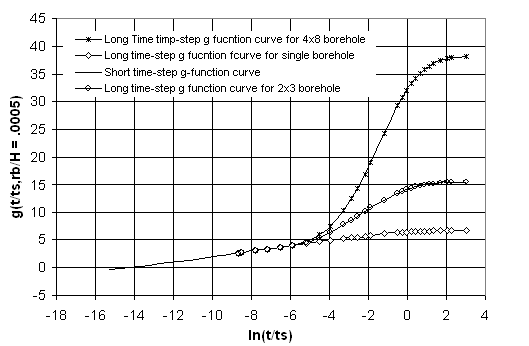
\includegraphics[width=0.9\textwidth, height=0.9\textheight, keepaspectratio=true]{media/image5651.png}
\caption{Short Time Step g Function Curve as an Extension of Long Time Step g Function Curves for Different Configuration of Boreholes (Eskilson 1987, Yavuzturk 1999). \protect \label{fig:short-time-step-g-function-curve-as-an}}
\end{figure}

The \emph{g}-functions developed by Eskilson are given only down to values of $\ln t/t_s = -4.5$, which for typical system and soil types can be on the order of 100 days. The values can be extended by the applying a line source model down to a time of $t = 5r_b^2/\alpha$. This time varies from 3-6 hours for a typical borehole field. This is because the analytical line source model, based on which the Eskilson model was developed, does not give a prompt increase in borehole wall temperature at \(r = {r_b}\) . It gives acceptable results only after the non-dimensional times of \(\alpha t/r_b^2 > 5\). But to model short time responses of a borehole we need response factors which can give accurate results down to minutes.

In order to generate the long time-step response functions on the fly, EnergyPlus has two different models that make two different approximations for the calculation of the response functions. The first model uses uniform heat flux boundary conditions (UHFcalc model) – that is, it assumes that all boreholes have the same uniform heat flux. The heat flux may vary over time, but it is always uniform throughout the field. The second model uses uniform borehole wall temperatures (UBHWTcalc model) – the heat flux will vary between boreholes and vary vertically for each borehole.

Calculation of \emph{g}-functions with uniform heat flux boundary conditions is simpler, but accuracy can decrease as the borehole-to-borehole interference increases. Consider a case with a large rectangular borefield, say 9x16 boreholes – if there is a significant annual imbalance in the heat rejection/heat extraction, the interior of the field will become thermally saturated, and the heat flux in the interior of the field will decrease over time. See Spitler, et al. (2020) for an illustration. The accuracy of using this approximation is discussed by Malayappan and Spitler (2013) with application to sizing of ground heat exchangers. As shown there, use of the UHFcalc model tends to overpredict the long-term temperature change for fields with significant borehole-to-borehole interference and significant annual heat rejection/heat extraction. In general, the UBHWTcalc model can be recommended for all applications, even though for a smaller numbers of boreholes the UHFcalc model offers sufficient accuracy.

For the UHFcalc model, EnergyPlus builds the model developed by Marcotte \& Pasquier(2009) which uses a discretized line source model. The \emph{g}-functions are generated using the following equation. The boreholes are discretized into segments. The temperature response of each segment on all other segments is then used to determine response factor for that particular geometry. The model estimates surface effects by creating ``imaginary" boreholes which are mirrored about the ground surface.

\begin{equation}
g = \frac{1}{2 H_T} \sum_{i=1}^N \sum_{j=1}^N \left( \int_{u_1^i}^{u_2^i} \int_{u_1^i}^{u_2^i} \frac{erfc\left( \frac{d(u_i, u_j)}{2\sqrt{\alpha t}}\right)}{d(u_i, u_j)} - \frac{erfc\left( \frac{d(u_i, u_j^{'})}{2\sqrt{\alpha t}}\right)}{d(u_i, u_j^{'})}\right)
\end{equation}

where:

\(N\) is the number of boreholes

\(H_T\) is the length of borehole

\(\alpha\) is the ground thermal diffusivity

\(t\) is the simulation time

\(u_1\) is the starting discretization point for borhole

\(u_2\) is the final discretization point for borehole

\(d(u_i, u_j)\) is the distance between current point and point on other borehole

\(d(u_i, u_j^{'})\) is the distance between current point and point on other imaginary borehole.

For the UBHWTcalc model, EnergyPlus builds on the model developed by Cimmino (2018a, 2018b, 2019), with improvements (Cook and Spitler 2021) to reduce memory consumption and increase speed. The general approach is similar to that of the UHFcalc model, but the heat flux is adjusted for each segment to enforce the uniform borehole wall temperature model. Additionally, the methodology of Cimmino (UBHWTcalc) is a semi-analytical solution, so the solution is dependent on the number of segments used. The number of segments are adaptively discretized to approximate a uniform inlet fluid temperature (UIFT) \emph{g}-function. 

Cimmino (2015) introduced a UIFT \emph{g}-function calculation that most closely matches physical reality. As boreholes are usually plumbed in parallel, the entering fluid temperatures are approximately uniform, and the actual distribution of heat within the field then depends on both the heat transfer outside the borehole and the heat transfer within the borehole. Thus, the g-function calculated with the UIFT boundary conditions depends on the flow rate and borehole thermal resistance in addition to the geometric configuration of the boreholes. Like, the UBHWT \emph{g}-function calculation, the UIFT calculation also depends on the number of segments used – as the number of segments used increases, the solution converges. 

So, though it’s possible to find a converged solution for the UIFT \emph{g}-function, it strictly speaking only applies when the borehole thermal resistance and flow rate remain fixed. Both commonly change during the system operation, as changing fluid temperatures affect the fluid properties. Therefore, the UIFT solution might be thought of as having a range of g-functions that change slightly with time. Therefore, in much the same way that radiation heat transfer within a zone is modeled with simplified methods because the occupants are likely to move the furniture, the UBHWT calculation can be used as a reasonable approximation to the UIFT calculation. As shown by Spitler, et al. (2020) the UIFT \emph{g}-function can closely match the UIFT \emph{g}-function, with considerably fewer segments. The number of segments required to closely approximate the UIFT \emph{g}-function varies with the number of boreholes and the borehole depth. Therefore, the UBHWT model uses an adaptive discretization algorithm that uses a smaller number of segments than the UIFT calculation. This provides excellent accuracy while requiring less computational time and memory. 

\subsubsection{Short Time-Step Response Factors}\label{short-time-step-response-factors}

The short timestep response is calculated by applying the model developed by Xu and Spitler (2006). This model maps the 2D geometry of the borehole onto a 1D radial geometry which preserves the thermal mass of the system, including the fluid. The multipole method (Claesson and Helstr{\"o}m, 2011) is used to correct the conductivity of the pipe and grout so the correct borehole resistance is maintained. The temperature response of the 1D domain is solved using a finite volume approach. The temperature at the borehole wall is then used to compute the g-function for short time-steps.

\subsubsection{Description of the Load Aggregation Scheme}\label{description-of-the-load-aggregation-scheme}

A load aggregation scheme was developed for energy simulation software with variable short time steps down to one minute. A major issue in the development was the calculation of the \emph{g}-functions.~ As discussed previously in the variable time step environments, the time step increments are not uniform. As a result, g-functions cannot e pre-calculated. Figure~\ref{fig:schematic-of-variable-time-step-model-g} shows a schematic of the variable time step ground loop heat exchanger model. The figure shows the larger monthly block loads, hourly loads and sub hourly loads and along with the time of occurrence of those loads. The figure also shows the time at which the \emph{g}-functions are applied to different load blocks.

\begin{figure}[hbtp] % fig 255
\centering
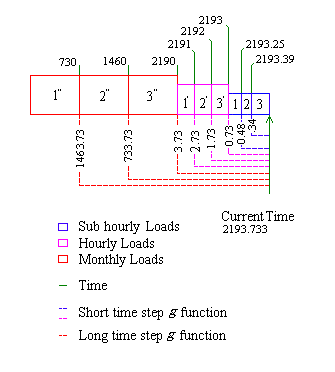
\includegraphics[width=0.9\textwidth, height=0.9\textheight, keepaspectratio=true]{media/image5656.png}
\caption{Schematic of Variable Time Step Model \emph{g} Function Calculation. \protect \label{fig:schematic-of-variable-time-step-model-g}}
\end{figure}

To calculate the response of a past load on the borehole temperature we apply the \emph{g}-function corresponding to the time elapsed since the load was applied. This is easily understood form the schematic. For example, to calculate the response of the aggregated load 1'' (at the end of 730hrs.) for the current time step (2193.733hrs) we apply a \emph{g}-function at 1463.73hrs. The \emph{g}-function for the same block 1'' at the previous time step, which occurred at 2193.25 hrs, would be at 1463.25hrs. From the schematic it is also seen that for the other two aggregated monthly loads 2'', 3'' the \emph{g}-function are applied at 733.73 hrs and 3.73 hrs for the current time-step and at 733.25 hrs and 3.25 hrs respectively for the previous time-step. The same scheme applies to hourly and sub-hourly. Thus to estimate the time at which the past monthly, hourly or sub-hourly loads occur, we might be tempted to store the simulation times at each time step for the entire simulation, storing load times for the whole length of simulation for a multi year simulation with a variable short time step would require a large amount of memory. But little consideration shows that it is not necessary.~ Since the monthly and hourly loads occur at equal intervals of time 730hrs and 1hr respectively, the \emph{g}-functions can be estimated with the current simulation time and the time at which the load block ends, which is a multiple of the monthly duration of the block size. Only the sub-hourly loads require storage of simulation times.

For example from the schematic (Figure~\ref{fig:schematic-showing-the-calculation-of-hourly}), for the sub hourly load 1, which occurred at the end of 2193.25 a \emph{g}-function at .48 hrs has to be applied and for the next load 2 a \emph{g}-function at 0.34 hrs has to be applied. Since the time intervals are not even for the sub hourly loads, we need to store the time steps at which those loads occurred. These times are required to estimate the time elapsed between the current simulation time and the time at which the sub hourly loads occurred.

Thus, the algorithm keeps track of the sub hourly loads along with their time of occurrence for a user-defined length of time during which the sub hourly calculations are made. The algorithm also estimates the time weighted hourly load from their corresponding sub hourly loads as each hour passes. The sub-hourly loads are time weighted because of the irregular intervals at which the time-step occurs. This is also illustrated in Figure~\ref{fig:schematic-showing-the-calculation-of-hourly}. The sub hourly loads 1,2 \&3 occur for varying length of time. The load 3 occurs for a longer duration than 1 and 2 in that order. This implies that the load 3 has to be given more weight than 1 and 2. So the sub hourly loads for a particular hour are multiplied by the length of their respective period of occurrence and averaged over the hour. This is further explained by the schematic in Figure~\ref{fig:simplified-single-zone-draw-through-air}.

\begin{figure}[hbtp] % fig 256
\centering
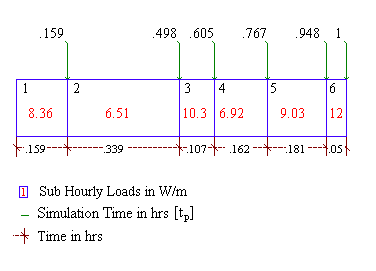
\includegraphics[width=0.9\textwidth, height=0.9\textheight, keepaspectratio=true]{media/image5657.png}
\caption{Schematic Showing the Calculation of Hourly Load from the Sub Houly Loads. \protect \label{fig:schematic-showing-the-calculation-of-hourly}}
\end{figure}

The bottom text in the boxes represents the magnitude of the sub hourly loads in W/m for each time step. The duration of the occurrence of each time-step for the each block is shown below the respective block. The first hourly load is given by the expression:

\begin{equation}
{\overline q_1} = \left[ \begin{array}{l}\left( {8.36 \times .159} \right) + \left( {6.51 \times .339} \right) + \left( {10.3 \times .107} \right)\\ + \left( {6.92 \times .162} \right) + \left( {9.03 \times .181} \right) + \left( {12 \times .05} \right)\end{array} \right] = 7.993W/m
\end{equation}

where \({\overline q_1}\) is the first hourly load (W/m).

The algorithm keeps track of enough of these past hourly loads to calculate the monthly load. As each month or user defined time passes, hourly loads over the entire month or user defined time ``blocks'' are averaged and stored in arrays for the respective monthly user defined block of time.

The borehole temperature for any time step is computed by superposing the monthly (larger time block loads) hourly and sub-hourly loads for each time step. To understand more clearly consider the schematic in Figure~\ref{fig:schematic-showing-the-calculation-of-hourly} where the borehole temperature at 2193.733 hour is to be estimated. Here the monthly block time is 730 hrs. We have three monthly aggregated load blocks for 730 hrs, 1460 hrs and 2190 hrs and hourly loads from 2191\(^{st}\) hr to 2193\(^{rd}\) hour. For the remaining 0.733 hours a sub hourly calculation is done. The three monthly aggregated load blocks when superposed using long time \emph{g-}functions, yields the borehole temperature at the end of 2190\(^{th}\) hour. Then the hourly loads from 2191\(^{st}\) to 2193\(^{rd}\) hrs are superposed using the corresponding short time step \emph{g} functions values yielding the borehole temperature at the end of 2193\(^{rd}\) hour. The sub-hourly variations for the current hour are obtained, by superposing the sub-hourly loads. From the schematic, we see there are two sub-hourly loads, 1 and 2. Thus the borehole temperature at the end of 2193.733 is expressed as:

\begin{equation}
{T_{2193.733}} = {T_{ground}} + \sum\limits_{m = 1}^3 {\left[ {\frac{{{{\overline{\overline q} }_m} - {{\overline{\overline q} }_{m - 1}}}}{{2\pi {k_{ground}}}}g\left( {\frac{{{t_{2193.733}} - {t_{730(m - 1)}}}}{{{t_s}}},\frac{{{r_b}}}{H}} \right)} \right]}
\end{equation}

\begin{equation}
+ \sum\limits_{n = 2190}^{2193} {\left[ {\frac{{{{\overline q }_n} - {{\overline q }_{n - 1}}}}{{2\pi {\kappa_{ground}}}}g\left( {\frac{{{t_{2193.733}} - {t_{n - 1}}}}{{{t_s}}},\frac{{{r_b}}}{H}} \right)} \right]}
\end{equation}

\begin{equation}
+ \sum\limits_{p = 2193}^{2193.733} {\left[ {\frac{{{q_p} - {q_{p - 1}}}}{{2\pi {\kappa_{ground}}}}g\left( {\frac{{{t_{2193.733}} - {t_p}}}{{{t_s}}},\frac{{{r_b}}}{H}} \right)} \right]}
\end{equation}

where:

\(\overline{\overline q}\) is the average monthly loads

\(\overline q\) is the average hourly loads

\emph{Q} is the sub-hourly loads

\emph{m} is the index for monthly aggregated blocks

\emph{p} is the array index for sub hourly loads

\emph{t} is time

t\(_{p}\) is the sub hourly time steps over the history period (here, the increment is not always unity).

Superposing the temperature responses of monthly (larger) blocks over the shorter, namely the hourly and sub hourly, introduces some error in the borehole temperature calculation at the beginning of every month. Yavuzturk and Spitler suggest a method to reduce the error in borehole temperature prediction by using a minimum hourly history period during which only the short time step superposition is carried out. In our model this idea is extended to sub hourly loads as well. Thus a user specified minimum sub-hourly history period is included along with the minimum hourly history period to model the sub-hourly variations. During this period only sub-hourly and hourly superpositions are made. This guarantees that at any given time step the superposition of temperature responses involves a minimum period of short time responses, which ensures a better estimation of borehole temperature. For example, a minimum hourly history period of 96 hrs and a minimum sub hourly history period of 5 hours would result in only 2 monthly aggregation blocks (1'' and 2''). The last monthly aggregation does not occur because neither of the minimum hourly history period of 96 hours or sub-hourly history period of five hrs is met. So an hourly superposition of the load is carried out for the third month until the minimum sub-hourly history period after which sub hourly superposition is carried out. The equation becomes

\begin{equation}
{T_{2193.733}} = {T_{ground}} + \sum\limits_{m = 1}^2 {\left[ {\frac{{{{\overline{\overline q} }_m} - {{\overline{\overline q} }_{m - 1}}}}{{2\pi {k_{ground}}}}g\left( {\frac{{{t_{2193.733}} - {t_{730(m - 1)}}}}{{{t_s}}},\frac{{{r_b}}}{H}} \right)} \right]}
\end{equation}

\begin{equation}
+ \sum\limits_{n = 1460}^{2188} {\left[ {\frac{{{{\overline q }_n} - {{\overline q }_{n - 1}}}}{{2\pi {\kappa_{ground}}}}g\left( {\frac{{{t_{2193.733}} - {t_{n - 1}}}}{{{t_s}}},\frac{{{r_b}}}{H}} \right)} \right]}
\end{equation}

\begin{equation}
+ \sum\limits_{p = 2188}^{2193.733} {\left[ {\frac{{{q_p} - {q_{p - 1}}}}{{2\pi {\kappa_{ground}}}}g\left( {\frac{{{t_{2193.733}} - {t_p}}}{{{t_s}}},\frac{{{r_b}}}{H}} \right)} \right]}
\end{equation}

Yavuzturk and Spitler have done a detailed analysis on the effect of minimum hourly history period. They found that a minimum hourly history period of 192 hrs for an annual simulation would reduce the running time by 90\%.~ They also found that for a 20-year simulation, the computation time of the aggregated load scheme is just 1\% of the non-aggregated load scheme.

\subsubsection{Summary of Variable Short Time Step Response Factor Model}\label{summary-of-variable-short-time-step-response-factor-model}

The load aggregation scheme developed in line with the above example is summarized eight steps as follows:

\begin{enumerate}
\item Define monthly load blocks duration (mb) in hrs (generally 730 hrs) and the minimum hourly history period and minimum sub hourly history period.
\item Read Borehole Geometry Parameters: number of boreholes, borehole length radius thickness of the pipe etc. Read Ground and Fluid thermal properties: Ground conductivity, volumetric specific heat capacity of the ground and heat carrier fluid. Read the short and long time-step \emph{g-}functions into arrays with their respective non-dimensionalized times.
\item Start Simulation from p = 1 to nts. Here ``nts'' is the number of time steps that have occurred since the start of simulation. (Note that P in not a count of number of hour elapsed in the simulation)
\item Compute the hourly loads as each hour passes. This is done by averaging the sub hourly loads during the past hour. The monthly loads are calculated by averaging the hourly loads during that month. This is done by summing the hourly loads during that monthly period and dividing the sum by 730 hours NumMonths(the number of months used in aggregation calculations) is set to the number of months of simulation (current number of aggregated load blocks)
\item If the simulation time is less than the minimum sub hourly history period the borehole temperature is estimated with no aggregation. Only sub hourly loads are superposed as given by the following equation.
\end{enumerate}

\begin{equation}
{T_{nts}} = {T_{ground}} + \sum\limits_{p = 1}^{nts} {\left[ {\frac{{{q_p} - {q_{p - 1}}}}{{2\pi {\kappa_{ground}}}}g\left( {\frac{{{t_{nts}} - {t_p}}}{{{t_s}}},\frac{{{r_b}}}{H}} \right)} \right]}
\label{eq:Tnts605}
\end{equation}

\begin{enumerate}
\setcounter{enumi}{5}
\item If the simulation time is less than sum of minimum hourly history and sub hourly history periods, then decomposed hourly aggregated loads are superposed using their corresponding g function until the sub hourly history required. Then the sub hourly temperature differences are found by superposing the decomposed sub hourly loads with their short time step \emph{g} functions. Average borehole temperature is found by superposing the hourly and sub hourly temperature differences with the following equation
\end{enumerate}

\begin{equation}
{T_{nts}} = \sum\limits_{n = 1}^{nh - sh} {\left[ {\frac{{{{\overline q }_n} - {{\overline q }_{n - 1}}}}{{2\pi {\kappa_{ground}}}}g\left( {\frac{{{t_{nts}} - {t_{n - 1}}}}{{{t_s}}},\frac{{{r_b}}}{H}} \right)} \right]}  + \sum\limits_{p = nts - sh}^{nts} {\left[ {\frac{{{q_p} - {q_{p - 1}}}}{{2\pi {\kappa_{ground}}}}g\left( {\frac{{{t_{nts}} - {t_p}}}{{{t_s}}},\frac{{{r_b}}}{H}} \right)} \right]}
\label{eq:Tnts606}
\end{equation}

\begin{enumerate}
\setcounter{enumi}{6}
\item If the simulation time is greater then the sum of a monthly period, sub hourly history and the hourly history period. Then monthly load aggregation is performed. Here if the difference between the simulation time and product of a monthly block period and the current number of monthly blocks is greater than the sum of the minimum hourly history and sub hourly history periods then the average borehole temperature is found by the following equation.
\end{enumerate}

\begin{equation}
\begin{array}{rl}
T_{nts} =& T_{ground} + \sum\limits_{m=1}^{calb} \left[ \frac{\overline{\overline q}_m - \overline{\overline q}_{m - 1}}{2\pi \kappa_{ground}} g \left( \frac{t_{nts} - t_{mb[m - 1]}}{t_s},\frac{r_b}{H} \right) \right] \\
 & + \sum\limits_{n = nh - [calb(mb) + sh]}^{nh - sh} {\left[ {\frac{{{{\overline q }_n} - {{\overline q }_{n - 1}}}}{{2\pi {\kappa_{ground}}}}g\left( {\frac{{{t_{nts}} - {t_{n - 1}}}}{{{t_s}}},\frac{{{r_b}}}{H}} \right)} \right]} \\
 & + \sum\limits_{p = nts - sh}^{nts} {\left[ {\frac{{{q_p} - {q_{p - 1}}}}{{2\pi {\kappa_{ground}}}}g\left( {\frac{{{t_{nts}} - {t_p}}}{{{t_s}}},\frac{{{r_b}}}{H}} \right)} \right]}
\end{array}
\label{eq:Tnts607}
\end{equation}

\begin{enumerate}
\setcounter{enumi}{7}
\item If the difference between the simulation time and product of a monthly block period and the current number of monthly blocks is less than the sum of the minimum hourly history and sub hourly history periods, then NumMonths is set to one month less than the actual number of months of simulation completed. The average borehole temperature is calculated by superposing the long and time step temperature differences using the following equation.
\end{enumerate}

\begin{equation}
\begin{array}{rl}
{T_{nts}} =& {T_{ground}} + \sum\limits_{m = 1}^{calb - 1} {\left[ {\frac{{{{\overline{\overline q} }_m} - {{\overline{\overline q} }_{m - 1}}}}{{2\pi {\kappa_{ground}}}}g\left( {\frac{{{t_{nts}} - {t_{mb[m - 1]}}}}{{{t_s}}},\frac{{{r_b}}}{H}} \right)} \right]} \\
 & + \sum\limits_{n = nh - [(calb - 1)(mb) + sh]}^{nh - sh} {\left[ {\frac{{{{\overline q }_n} - {{\overline q }_{n - 1}}}}{{2\pi {\kappa_{ground}}}}g\left( {\frac{{{t_{nts}} - {t_{n - 1}}}}{{{t_s}}},\frac{{{r_b}}}{H}} \right)} \right]} \\
 & + \sum\limits_{p = nts - sh}^{nts} {\left[ {\frac{{{q_p} - {q_{p - 1}}}}{{2\pi {\kappa_{ground}}}}g\left( {\frac{{{t_{nts}} - {t_p}}}{{{t_s}}},\frac{{{r_b}}}{H}} \right)} \right]}
\end{array}
\label{eq:Tnts608}
\end{equation}

The following is a summary of the above eight steps:

Define Monthly block duration, minimum hourly history period and minimum sub hourly history period (\textbf{Step 1})

Read Borehole Geometry parameters, Ground and carrier fluid properties and read short and long time-step \emph{g} functions (\textbf{Step 2})

\textbf{Do until} p = 1 to number of time-steps (nts) (\textbf{Step 3})

Compute the Ground Load for the current time step using Entering Fluid temperature (For the first time-step \emph{T}\(_{FarField}\) may be used)

Compute the hourly loads as each hour and monthly loads as each month passes. Calculate the number of monthly blocks (NumMonths)(\textbf{Step 4})

~~~ \textbf{If} (Current time less than minimum sub hourly history) (\textbf{Step 5})

~~~ ~~~~~~ \textbf{~~~} use Equation~\ref{eq:Tnts605}

~~~ \textbf{Else If} (Current Simulation Time less than sum of minimum hourly history and minimum sub hourly history) (\textbf{step 6})

~~~ ~~~~~~ use Equation~\ref{eq:Tnts606}

~~~ \textbf{Else}

~~~ ~~~~~~ \textbf{If} (Difference between current simulation~~~ time and duration of the total number months is Greater than sum of minimum hourly and sub hourly histories) (\textbf{step 7})

~~~~~~~~~~~~~~~~~use Equation~\ref{eq:Tnts607}

~~~~~~~~~~ \textbf{Else} (\textbf{step 8})

~~~~~~~~~~~~~~~~~ use Equation~\ref{eq:Tnts608}

~~~ ~~~~~~ \textbf{End if}

~~~ \textbf{End if}

\textbf{End do}

\subsubsection{References}\label{references-2-006}

\hangindent=2em
\hangafter=1
\noindent Claesson, J., G. Helstr{\"o}m. 2011. Multipole method to calculate borehole thermal resistances in a borehole heat exchanger. HVAC\&R Research. 17(6), 895-911.

\hangindent=2em
\hangafter=1
\noindent Cook, J. C. and J. D. Spitler. 2021. Faster computation of g-functions used for modeling of ground heat exchangers with reduced memory consumption. Building Simulation 2021. Bruges, Belgium, IBPSA.

\hangindent=2em
\hangafter=1
\noindent Cimmino, M. (2015).``The effects of borehole thermal resistances and fluid flow rate on the g-functions of geo-thermal bore fields." International Journal of Heat and Mass Transfer 91: 1119-1127.

\hangindent=2em
\hangafter=1
\noindent Cimmino, M. 2018a. ``Fast calculation of the g-functions of geothermal borehole fields using similarities in the evaluation of the finite line source solution." Journal of Building Performance Simulation 11(6): 655-668.

\hangindent=2em
\hangafter=1
\noindent Cimmino, M. 2018b. pygfunction: an open-source toolbox for the evaluation of thermal. eSim 2018, Montreál, IBPSA Canada.

\hangindent=2em
\hangafter=1
\noindent Cimmino, M. 2019. ``Semi-Analytical Method for g-Function Calculation of bore fields with series- and parallel-connected boreholes." Science and Technology for the Built Environment 25(8): 1007-1022.

\hangindent=2em
\hangafter=1
\noindent Eskilson, P. 1987. Thermal Analysis of Heat Extraction Boreholes. Ph.D.~Thesis, Department of Mathematical Physics, University of Lund, Lund, Sweden.

\hangindent=2em
\hangafter=1
\noindent Malayappan, V. and J. D. Spitler. 2013. Limitations of Using Uniform Heat Flux Assumptions in Sizing Vertical Borehole Heat Exchanger Fields. Clima 2013. Prague (Czech Republic).

\hangindent=2em
\hangafter=1
\noindent Spitler, J. D., J. C. Cook and X. Liu. 2020. A Preliminary Investigation on the Cost Reduction Potential of Optimizing Bore Fields for Commercial Ground Source Heat Pump Systems. Proceedings, 45th Workshop on Geothermal Reservoir Engineering. Stanford, California, Stanford University. 

\hangindent=2em
\hangafter=1
\noindent Spitler, J. D., J. C. Cook and X. Liu. 2020. FY20 Second Milestone Report for Advanced Techno-Economic Model-ing for Geothermal Heat Pump Applications in Residential, Commercial, and Industry Building, Oak Ridge Na-tional Laboratory.

\hangindent=2em
\hangafter=1
\noindent Xu, X., J.D. Spitler. 2006. Modeling of Vertical Ground Loop Heat Exchangers with Variable Convective and Thermal Mass of Fluid. Proceedings of the 10th International Conference on Thermal Energy Storage-Ecostock 2006, Pomona, NJ.

\hangindent=2em
\hangafter=1
\noindent Yavuzturk, C. 1999. Modeling of Vertical Ground Loop Heat Exchangers for Ground Source Heat Pump Systems. Ph.D.~Thesis, Department of Mechanical and Aerospace Engineering, Oklahoma State University, Stillwater, Oklahoma.

\hangindent=2em
\hangafter=1
\noindent Yavuzturk, C., J.D. Spitler. 1999. A Short Time Step Response Factor Model for Vertical Ground Loop Heat Exchangers. ASHRAE Transactions. 105(2):475-485.

\subsection{GroundHeatExchanger:Slinky}\label{groundheatexchangerslinky}

This model reuses much of the same code including the load aggregation and temperature response caluclations which are described above in the GroundHeatExchanger:Vertical model. As a result, that section can also be used as reference material. This model is unique in that it generates it's own temperature response factor g-functions, rather than relying on the other software or data to generate the g-functions. These are generated based on the work by Xiong et al. 2015.

\subsubsection{Horizontal Slinky Temperature Response Functions}\label{horizontal-slinky-temperature-response-functions}

Equation used for calculating the g-function temperature response factors for the horizontal Slinky HX are seen below.

{\scriptsize
\begin{equation}
g_s\left(t\right) = \sum_{i = 1}^{N_{ring}} \sum_{j = 1}^{N_{ring}} \frac{R}{4\pi N_{ring}} \int_0^{2\pi} \int_0^{2\pi} 
            \left[ 
                \frac{erfc\left(d\left(P_j,P_i\right)/2\sqrt{\alpha t}\right)}{d\left(P_j,P_i\right)} - 
                \frac{erfc\left(\sqrt{d\left(P_j,P_i\right)^2+4h^2/\left(2\sqrt{\alpha t}\right)}\right)}{\sqrt{d\left(P_j,P_i\right)^2+4h^2} }
            \right]d\omega d\varphi
\end{equation}}

where:

\begin{equation}
d\left(P_j,P_i\right) = \frac{d\left(P_{ii},P_j\right) + d\left(P_{io},P_j\right)}{2}
\end{equation}

\begin{equation}
d\left(P_{ii},P_j\right) = \sqrt{\left[x_{0i} + \left(R-r\right)\cos \varphi - x_{0j}-R\cos \omega\right]^2 + \left[y_{0i} + \left(R-r\right)\sin \varphi - y_{0j}-R\sin \omega\right]^2}
\end{equation}

\begin{equation}
d\left(P_{io},P_j\right) = \sqrt{\left[x_{0i} + \left(R-r\right)\cos \varphi - x_{0j}-R\cos \omega\right]^2 + \left[y_{0i} + \left(R+r\right)\sin \varphi - y_{0j}-R\sin \omega\right]^2}
\end{equation}

\subsubsection{Vertical Slinky Temperature Response Functions}\label{vertical-slinky-temperature-response-functions}

Equations used for calculating the g-function temperature response factors for the vertical Slinky HX are seen below.

\begin{equation}
g_s\left(t\right) = \sum_{i = 1}^{N_{ring}} \sum_{j = 1}^{N_{ring}} \frac{R}{4\pi N_{ring}} \int_0^{2\pi} \int_0^{2\pi} 
            \left[ 
                \frac{erfc\left(d\left(P_j,P_i\right)/2\sqrt{\alpha t}\right)}{d\left(P_j,P_i\right)} - 
                \frac{erfc\left(d\left(P_{j'},P_i\right)/2\sqrt{\alpha t}\right)}{d\left(P_{j'},P_i\right)}
            \right]d\omega d\varphi
\end{equation}

where:

\begin{equation}
d\left(P_j,P_i\right) = \frac{d\left(P_{ii},P_j\right) + d\left(P_{io},P_j\right)}{2}
\end{equation}

\begin{equation}
d\left(P_{j'},P_i\right) = \frac{d\left(P_{ii},P_{j'}\right) + d\left(P_{io},P_{j'}\right)}{2}
\end{equation}

{\scriptsize
\begin{equation}
d\left(P_{ii},P_j\right) = \sqrt{\left[x_{0i} + \left(R-r\right)\cos \varphi - x_{0j}-R\cos \omega\right]^2 + \left[y_{0i}-y_{0j}\right]^2 + \left[z_{0i} + \left(R-r\right)\sin \varphi - z_{0j}-R\sin \omega\right]^2}
\end{equation}}

{\scriptsize
\begin{equation}
d\left(P_{io},P_j\right) = \sqrt{\left[x_{0i} + \left(R+r\right)\cos \varphi - x_{0j}-R\cos \omega\right]^2 + \left[y_{0i}-y_{0j}\right]^2 + \left[z_{0i} + \left(R+r\right)\sin \varphi - z_{0j}-R\sin \omega\right]^2}
\end{equation}}

{\scriptsize
\begin{equation}
d\left(P_{ii},P_{j'}\right) = \sqrt{\left[x_{0i} + \left(R-r\right)\cos \varphi - x_{0j}-R\cos \omega\right]^2 + \left[y_{0i}-y_{0j}\right]^2 + \left[z_{0i} + \left(R-r\right)\sin \varphi - z_{0j} - 2h - R\sin \omega\right]^2}
\end{equation}}

{\scriptsize
\begin{equation}
d\left(P_{io},P_{j'}\right) = \sqrt{\left[x_{0i} + \left(R+r\right)\cos \varphi - x_{0j}-R\cos \omega\right]^2 + \left[y_{0i}-y_{0j}\right]^2 + \left[z_{0i} + \left(R+r\right)\sin \varphi - z_{0j} - 2h - R\sin \omega\right]^2}
\end{equation}}

\subsubsection{Model Simplifications for Computational Efficiency}\label{model-simplifications-for-computational-efficiency}

Several simplifications were used to ensure the g-function temperature response factors are computationally efficient. The first simplification is achieved by taking advantage of symmetry. In the Figure~\ref{fig:slinky-first-and-second-improvements} below, we can see that by taking advantage of symmettry the temperature response for only one quarter of the rings needs be calculated.

The second simplification occurs by realizing that the effect between two rings decreases exponentially as the distance between the rings increases. Near-field rings are defined as rings whose centers are within 2.5m + D distance from the center of ring i as is seen in Figure~\ref{fig:slinky-first-and-second-improvements}. Far-field rings are defined as rings whose centers are beyond 10m + D, with middle-field rings occupying the space in between the near-field and far-field rings. Near-field ring temperature response factors are determined as indicated above for horzontal or vertical slinkys. Middle-field rings are considerably simplified -- the interaction between ring is approximated as that of two point sources at their centers. Thermal effect of far-field rings are ignored.

The third and final simplification takes advantatge of geometric similarity that ring share. Ring pairs that are geometrically similar do not require recalculation of distances or reponse factors. Thus the calculations for geometrically similar ring pairs can be reused.

For more information, see the Xiong et al. (2015) reference listed below.

\begin{figure}[htbp]
\centering
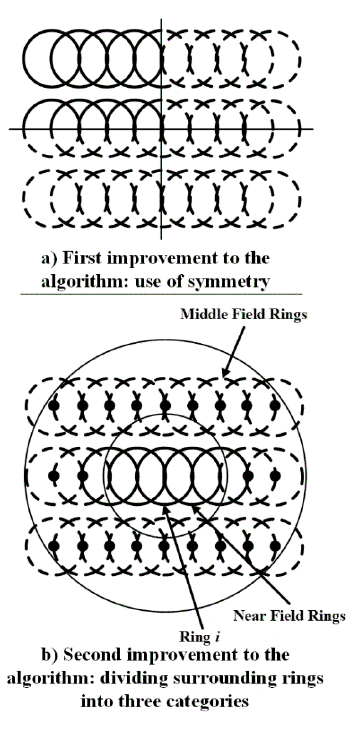
\includegraphics[width=0.5\textwidth]{media/image8001.png}
\caption{Schematic of first and second improvements to the algorithm for computational efficiency \protect \label{fig:slinky-first-and-second-improvements}}
\end{figure}

\subsubsection{References}\label{references-3-003}

Xiong, Z., D.E. Fisher, and J.D. Spitler. 2015. Development and Validation of a Slinky(TM) Ground Heat Exchanger Model. Applied Energy 141: 57-69.

\subsection{Plant Loop Pond-To-Water Heat Exchanger}\label{plant-loop-pond-to-water-heat-exchanger}

The pond model (Object: GroundHeatExchanger:Pond) is a `lumped parameter' model where the pond is represented by a single node with thermal mass. The pond surface temperature is the same as the temperature at this node, i.e.~the surface temperature is the same as the bulk temperature. A first order differential equation is solved in the model to calculate the pond temperature at each time step. This type of heat rejecter is modeled as several circuits connected in parallel.

\begin{figure}[hbtp] % fig 257
\centering
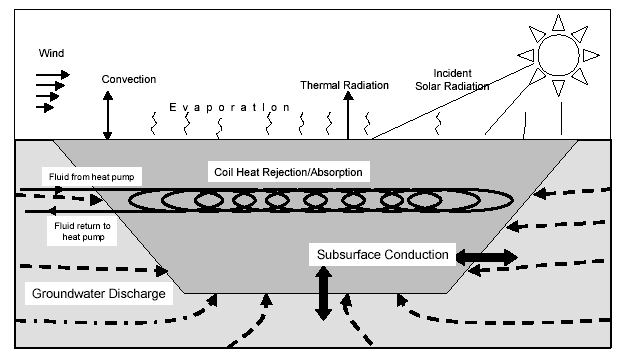
\includegraphics[width=0.9\textwidth, height=0.9\textheight, keepaspectratio=true]{media/image5676.png}
\caption{Heat Transfer Mechanisms in a Pond (Chiasson 1999) \protect \label{fig:heat-transfer-mechanisms-in-a-pond-chiasson}}
\end{figure}

Rees (2002) implemented the model developed by Chiasson (1999) for the shallow ponds. The model is based on the assumption that thermal gradients in shallow ponds are negligible, especially during times of heat rejection. Using the lumped parameter approach, an overall energy balance for the pond may be devised as:

\begin{equation}
q{}_{in} - q{}_{out} = V\rho C{}_p\frac{{dT}}{{dt}}
\end{equation}

where:

\(q{}_{in}\) is the heat transfer to the pond

\(q{}_{out}\) is the heat transfer from the pond

\(V\) is the pond volume

\(\rho\) is the density of pond water

\({q_{in}}\) is the heat transfer to the pond

\(C{}_p\) is the specific heat capacity of pond water

\(\frac{{dT}}{{dt}}\) is the  rate of change of temperature of the pond water.

The rate of change in average pond temperature is given as:

\begin{equation}
\frac{{dT}}{{dt}} = \frac{{q{}_{solar} + q{}_{thermal} + q{}_{convection} + q{}_{groundwater} + q{}_{evaporation} + q{}_{fluid}}}{{V\rho C{}_p}}
\end{equation}

where:

q\(_{solar}\) is the solar radiation heat gain to the pond

q\(_{thermal}\) is the thermal radiation heat transfer at the pond surface.

q\(_{convection}\) is the convection heat transfer at the pond surface

q\(_{ground}\) is the heat transfer to/from ground to the pond

q\(_{groundwater}\) is the heat transfer due to ground water inflow/outflow

q\(_{evaporation}\) is the heat transfer due to evaporation at the pond surface

q\(_{fluid}\) is the total heat transfer to/from the heat exchanging fluid flowing in all spools or~ coils in the pond.

A heat balance is calculated at a single node that represents the pond. Heat transfer takes place by surface convection, long-wave radiation to the sky, absorption of solar energy, ground heat transfer and heat exchange with the fluid. A heat exchanger analogy is used to calculate the heat transfer between the heat transfer fluid and the pond. The differential equation defined by the heat balance is solved using a fourth order Runge-Kutta numerical integration method. The implementation along with the model equations are summarized in the figure below.

\begin{figure}[hbtp] % fig 258
\centering
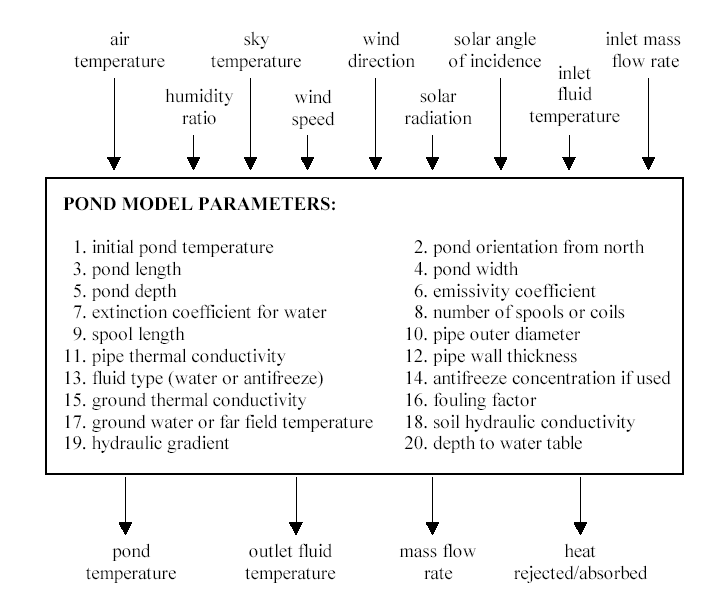
\includegraphics[width=0.9\textwidth, height=0.9\textheight, keepaspectratio=true]{media/image5686.png}
\caption{Pond Model Component Configuration (Chiasson 1999) \protect \label{fig:pond-model-component-configuration-chiasson}}
\end{figure}

The model overall pond model consists in a number of sub-models which are enumerated below.

\subsubsection{Solar radiation heat gain to the pond}\label{solar-radiation-heat-gain-to-the-pond}

\begin{equation}
\rho ' = {\tau_a} - \tau
\end{equation}

where:

\(\rho '\) is the reflectance

\(\tau\) ~is the transmittance of solar radiation by the pond surface and the subscript `a' refers to the absorbed component.

\begin{equation}
{\tau_a} = {e^{\frac{{ - \mu 'd}}{{\cos {\theta_r}}}}}
\end{equation}

and

\begin{equation}
\tau  = \frac{1}{2}\left( {\frac{{1 - {r_{par}}}}{{1 + {r_{par}}}} + \frac{{1 - {r_ \bot }}}{{1 + {r_ \bot }}}} \right){e^{\frac{{ - \mu 'd}}{{\cos {\theta_r}}}}}
\end{equation}

where:

\(\mu '\) is the extinction coefficient for water

\(d\) is the pond depth

\({r_{par}}\) represents the parallel component of unpolarized radiation and \({r_ \bot }\) represents the perpendicular component of unpolarized radiation which are computed by Duffie and Beckman (1991) as:

\begin{equation}
  r_{par} = \frac{\tan ^2 \left( \theta_r - \theta \right)}{\tan ^2 \left( \theta_r + \theta \right)}
\end{equation}

\begin{equation}
  r_{\bot} = \frac{\sin ^2 \left( \theta_r - \theta \right)}{\sin ^2 \left( \theta_r - \theta  \right)}
\end{equation}

Finally, the amount of solar radiation absorbed by the pond (\({q_{solar}}\)) is expressed as:

\begin{equation}
{q_{solar}} = I\left( {1 - \rho '} \right){A_{pond}}
\end{equation}

where:

\(I\) is the solar radiation flux incident on the pond surface (here, the total reflectance is approximated by the beam reflectance)

\({A_{pond}}\) is the area of the pond surface.

The model also accepts solar radiation in the form of beam \(\left( {{I_b}} \right)\) and diffuse \(\left( {{I_d}} \right)\) components, in which case \(I\) is computed from:

\begin{equation}
I = {I_b}\cos \theta  + {I_d}
\end{equation}

\subsubsection{Thermal radiation heat transfer at the pond surface}\label{thermal-radiation-heat-transfer-at-the-pond-surface}

\begin{equation}
q{}_{thermal} = \sigma \alpha (T{{}_{surface}^4} - T{{}_{sky}^4})
\end{equation}

where:

\(\alpha\) is the thermal absorptivity

\(\sigma\) is the Stefan Boltzman constant.

\subsubsection{Convection heat transfer at the pond surface}\label{convection-heat-transfer-at-the-pond-surface}

\begin{equation}
q{}_{convection} = h{}_c(T{}_{pond} - T{}_{db})
\end{equation}

ASHRAE simple convection coefficient model is used to obtain the convection coefficient for external surfaces. Initializing of pond temps to mean of dry-bulb temperature T\(_{db}\) and ground temperatures is useful because repeated warm up days tend to drive the initial pond temperature toward the dry-bulb temperature Hence, for each environment the simulation starts the pond temperature T\(_{pond}\) midway between the dry-bulb and ground temperature.

\subsubsection{Heat transfer to/from ground to the pond}\label{heat-transfer-tofrom-ground-to-the-pond}

Hull et al (1984) expressed the following equation for ground heat losses from any pond. The equations are also based on the assumption that, for all practical purposes, the constant temperature sink is the ground water table (Kishore and Joshi 1984):

\begin{equation}
q{}_{ground} = U{}_{ground}A{}_{ground}(T{}_{groundwater} - T{}_{pond})
\end{equation}

\begin{equation}
U{}_{ground} = 0.999\left( {\frac{{k{}_{ground}}}{{d{}_{groundwater} - d{}_{pond}}}} \right) + 1.37\left( {\frac{{k{}_{ground}P{}_{pond}}}{{A{}_{pond}}}} \right)
\end{equation}

where:

\(k{}_{ground}\) is the thermal conductivity of the ground

\(d{}_{groundwater}\) is the depth of water table

\(d{}_{pond}\) is the pond depth

\(P{}_{pond}\) is the pond perimeter.

\subsubsection{Heat transfer due to evaporation at the pond surface}\label{heat-transfer-due-to-evaporation-at-the-pond-surface}

Evaporation is calculated assuming a fixed Lewis number unlike the Chaisson model.

\begin{equation}
q{}_{evaporation} = {\left( {\frac{{\Pr }}{{Sc}}} \right)^{2/3}}\left( {\frac{{h{}_c}}{{C{}_{p,air}}}} \right)\left( {HR{}_f - HR{}_a} \right)\left( {q{}_l} \right)
\end{equation}

where:

\(Pr\) is the Prandtl number for air

\(Sc\) is the Schmidt number for air

\(h_c\) is the convection coefficient

\(HR_f\) is the humidity ratio at pond surface/film temperature

\(HR_a\) is the humidity ratio of air

\(q_l\) is the latent heat of air.

Air properties are obtained by applying the existing the psychometric functions of EnergyPlus.

\subsubsection{Total heat transfer to/from the heat exchanging fluid flowing in all spools or coils in the pond}\label{total-heat-transfer-tofrom-the-heat-exchanging-fluid-flowing-in-all-spools-or-coils-in-the-pond}

\begin{equation}
q{}_{fluid} = UA{}_{pipe}(T{}_{fluid} - T{}_{pond})N{}_{circuit}
\end{equation}

where:

\(UA{}_{pipe}\) is the overall heat transfer coefficient expressed in terms of inside pipe area

\(N{}_{circuit}\) is the number of spools installed in the pond.

The fluid temperature Tfluid is computed as the average fluid temperatures of the inlet and the outlet node at a given temperature.

\begin{equation}
U{A_{pipe}} = \frac{{2\pi {r_i}\cdot {L_{spool}}}}{{\sum {{r_t}} }}
\end{equation}

where:

\({r_i}\) is the inner pipe radius

\({L_{spool}}\)  is the length of one spool

\(\sum {{r_t}}\) is the composite thermal resistance defined as the resistance due to fluid flow in the pipe plus the external pipe thermal resistance plus the fouling factor.

\subsubsection{References}\label{references-4-002}

Chiasson, A.D. 1999. \emph{Advances in modeling of groundsourceheat pump systems}. Master's thesis,Oklahoma State University, Stillwater, OK

Duffie, J.A., and W.A. Beckman. 1991. \emph{Solar engineering of thermal processes,} 2d ed. New York: John Wiley \& Sons.

Hull, J.R., K.V. Liu, W.T. Sha, J. Kamal, and C.E. Nielsen. 1984. Dependence of ground heat losses upon solar pond size and perimeter insulation---Calculated and experimental results. \emph{Solar Energy} 33(1): 25-33

Kishore, V.V.N., and V. Joshi. 1984. A practical collector efficiency equation for nonconvecting solar ponds. \emph{Solar Energy} 33(5): 391-395.

Rees, S.J., J.D. Spitler and X. Xiao, X 2002.\href{http://www.hvac.okstate.edu/pdfs/Rees_Spitler_Xiao_02.pdf}{Transient Analysis of Snow-melting System Performance}.\emph{ASHRAE Transactions.}108(2):406-423.

\subsection{Plant Loop Surface-Ground-To-Water Heat Exchanger}\label{plant-loop-surface-ground-to-water-heat-exchanger}

This model (Object: GroundHeatExchanger:Surface) is based on the QTF formulation of heat transfer through building elements with embedded heat sources/sinks. The model uses a heat exchanger analogy to relate the inlet fluid temperature to the net heat transfer rate and consequently outlet temperature. The model is entirely passive, i.e.~it does not set any flow rates or incorporate any controls. In order to deal with the non-linear boundary conditions at the top surface due to the presence of ice/snow fluxes have to be calculated by the QTF model and temperature calculated from the surface heat balance. This requires some iteration. Note, top surface variables correspond to `outside' variables in standard CTF/QTF definition. Bottom surface variables correspond to `inside' variables.

For given current surface temperatures the terms of the QTF equations can be grouped into constant terms, and those depending on the current source flux. The surface heat balance may be given by the following equation (Strand, 1997):

\begin{equation}
QS{}_{} = \sum\limits_{m = 1}^M {X{}_{k,m}} T{}_{i,t - m + 1} - \sum\limits_{m = 1}^M {Y{}_{k,m}} T{}_{o,t - m + 1} + \sum\limits_{m = 1}^k {F{}_m} q{}_{i,t - m} + \sum\limits_{m = 1}^M {W{}_m} {q''}{}_{source,t - m + 1}
\end{equation}

\begin{equation}
T{}_S{}_{} = \sum\limits_{m = 1}^M {X{}_{k,m}} T{}_{i,t - m + 1} - \sum\limits_{m = 1}^M {Y{}_{k,m}} T{}_{o,t - m + 1} + \sum\limits_{m = 1}^k {F{}_m} q{}_{i,t - m} + \sum\limits_{m = 1}^M {W{}_m} q''{}_{source,t - m + 1}
\end{equation}

where:

T\(_{s}\) is the temperature of the node where the heat source or sink is present

\(QS\) is the surface heat balance

\({q''_{source}}\) is the heat flux at the location of the heat source or sink

\(T\)is the temperature

\(i\) is the inside of the building element

\(o\) is the outside of the building element

\(t\) is the current time step

\(X,~Y,~F,~W\) are conduction transfer functions.

The surface balance equation includes terms for incident solar energy, radiation heat transfer from internal sources, linearized radiation between surfaces using the mean radiation temperature concept and convection to the surrounding air.

The heat balance on the water loop is given by:

\begin{equation}
q = \dot mc{}_p(T{}_{wi} - T{}_{wo})
\end{equation}

where:

\(q\) is the heat transferred between the water loop and the building elements

\(\dot m\) is the mass flow rate of water

\(T{}_{wi}\) is the inlet water temperature

\(T{}_{wo}\) is the outlet water temperature.

From the second law of thermodynamics the maximum amount of heat transfer is:

\begin{equation}
q{}_{\max } = (\dot mc{}_p){}_{water}(T{}_{wi} - T{}_s)
\end{equation}

where \(T_{s}\) = temperature at the source location

The effectiveness of the heat exchanger is given by:

\begin{equation}
\varepsilon  = 1 - {e^{ - NTU}}
\end{equation}

where NTU is defined by:

\begin{equation}
NTU = \frac{{UA}}{{(\dot mC{}_p){}_{water}}}
\end{equation}

and

\begin{equation}
UA = h\pi DL
\end{equation}

where h is the convection coefficient, D is the interior tube diameter, and L is the total length of the tube.

The Colburn equation is used to define the Nusselt number Nu:

\begin{equation}
Nu = \frac{{hD}}{k} = 0.023{{Re}_D^{4/5}}{Pr^{1/3}}
\end{equation}

where Pr is the Prandtl number, Re is the Reynolds number and k is the thermal conductivity of the fluid.

\begin{equation}
{Re}_D = \frac{{4\dot m}}{{\pi \mu D}}
\end{equation}

where \(\mu\) is the absolute viscosity of water.

\subsection{Plant Loop Fluid-to-Fluid Heat Exchanger}\label{plant-loop-fluid-to-fluid-heat-exchanger}

This component (Object: HeatExchanger:FluidToFluid) is a simple hydronic heat exchanger that can be used to couple two (hydronic) plant or condenser loops.~ Sizing and nominal capacity calculations are discussed elsewhere in this document, see the section called Plant Heat Exchanger Sizing. This section first discusses the heat transfer modeling and the control issues.

Heat exchanger performance modeling uses classic effectiveness-NTU correlations. The heat exchanger model can be specified as one of seven types: ~cross flow both fluid streams unmixed, cross flow both fluid streams mixed, cross flow Loop Supply Side mixed and Loop Demand Side unmixed, cross flow Loop Supply Side unmixed and Loop Demand Side mixed, counter flow, parallel flow, or ideal. The model correlations determine a heat transfer effectiveness value, \(\varepsilon\), which is a function of heat exchanger UA, the mass flow rates through boths sides, and the specific heat of the fluids in the streams.~ The effectiveness of an ideal heat exchanger is set to 1.0 and no correlation is needed.

Because the heat exchanger is intended to be generic, its two sides are distinguished by the nature of loop side being connected.~ One side is called ``Loop Supply Side'' to indicate the heat exchanger is situated on the supply side of a loop. The other side is called ``Loop Demand Side'' to indicate it is on the demand side of a loop.~ The heat exchanger is intended to act as a supply component for the loop connected to it as the ``Loop Supply Side'' and as a demand component for the loop connected to it as the ``Loop Demand Side.''~ From the point of view of the heat exchanger component itself, the Loop Demand Side acts like a supply source/sink for the Loop Supply Side which acts like a demand to the component.

The mass flow rates and specific heat capacity are multiplied together to evaluate flow thermal capacity for each side and the minimum, maximum, and capacity ratio, \({R_C}\), are determined.

\begin{equation}
{\left( {\dot m{c_p}} \right)_{SupLoop}} = {\dot m_{SupLoop}}*{c_p}_{SupLoop}
\end{equation}

\begin{equation}
{\left( {\dot m{c_p}} \right)_{DmdLoop}} = {\dot m_{DmdLoop}}*{c_p}_{DmdLoop}
\end{equation}

\begin{equation}
{\left( {\dot m{c_p}} \right)_{Min}} = MIN\left( {{{\left( {\dot m{c_p}} \right)}_{SupLoop}},{{\left( {\dot m{c_p}} \right)}_{DmdLoop}}} \right)
\end{equation}

\begin{equation}
{\left( {\dot m{c_p}} \right)_{Max}} = MAX\left( {{{\left( {\dot m{c_p}} \right)}_{SupLoop}},{{\left( {\dot m{c_p}} \right)}_{DmdLoop}}} \right)
\end{equation}

\begin{equation}
{R_C} = \frac{{{{\left( {\dot m{c_p}} \right)}_{Min}}}}{{{{\left( {\dot m{c_p}} \right)}_{Max}}}}
\end{equation}

NTU, or Number of Transfer Units, is calculated using:

\begin{equation}
NTU = \frac{{UA}}{{{{\left( {\dot m{c_p}} \right)}_{Min}}}}
\end{equation}

For a counter flow heat exchanger, effectiveness is calculated using:

\begin{equation}
\varepsilon  = \frac{{1 - exp\left[ { - NTU\left( {1 - {R_C}} \right)} \right]}}{{1 - {R_C}exp\left[ { - NTU\left( {1 - Rc} \right)} \right]}}
\end{equation}

For a parallel flow heat exchanger, effectiveness is calculated using:

\begin{equation}
\varepsilon  = \frac{{1 - exp\left[ { - NTU\left( {1 + {R_C}} \right)} \right]}}{{\left( {1 + {R_C}} \right)}}
\end{equation}

For a cross flow heat exchanger with both streams unmixed, effectiveness is calculated using:

\begin{equation}
\varepsilon  = 1 - exp\left\{ {\frac{{NT{U^{0.22}}}}{{{R_C}}}\left[ {exp\left( { - {R_C}NT{U^{0.78}}} \right) - 1} \right]} \right\}
\end{equation}

For a cross flow heat exchanger with both streams mixed, the effectiveness is calculated using:

\begin{equation}
\varepsilon  = {\left[ {\frac{1}{{1 - exp\left( { - NTU} \right)}} + \frac{{{R_C}}}{{1 - exp\left( { - {R_C}NTU} \right)}} - \frac{1}{{NTU}}} \right]^{ - 1}}
\end{equation}

For a cross flow heat exchanger with the stream with the higher capacity mixed and the stream with the lower capacity unmixed, the effectiveness is calculated using:

\begin{equation}
\varepsilon  = \frac{1}{{{R_C}}}\left\{ {1 - exp\left[ {{R_C}\left( {exp\left( { - NTU} \right) - 1} \right)} \right]} \right\}
\end{equation}

For a cross flow heat exchanger with the stream with higher capacity unmixed and the stream with lower capacity mixed, the effectiveness is calculated using:

\begin{equation}
\varepsilon  = 1 - exp\left\{ { - \frac{1}{{{R_C}}}\left[ {1 - exp\left( { - {R_C}NTU} \right)} \right]} \right\}
\end{equation}

Effectiveness values are always limited to be no higher than 1.0.~ The program code protects from evaluating the exponential with operands that are too large or too small. Once the effectiveness value is determined, the heat transfer rate is calculated using:

\begin{equation}
\dot Q = \varepsilon {\left( {\dot m{c_p}} \right)_{Min}}\left( {{T_{SupLoop,In}} - {T_{DmdLoop,In}}} \right)
\end{equation}

Lastly, the fluid temperatures leaving the heat exchanger are calculated using:

\begin{equation}
{T_{SupLoop,Out}} = {T_{SupLoop,In}} - \frac{{\dot Q}}{{{{\left( {\dot m{c_p}} \right)}_{SupLoop}}}}
\end{equation}

\begin{equation}
{T_{DmdLoop,Out}} = {T_{DmdLoop,In}} + \frac{{\dot Q}}{{{{\left( {\dot m{c_p}} \right)}_{DmdLoop}}}}
\end{equation}

The plant heat exchanger offers a number of control options for a wide variety of applications.~ This section documents the control decision logic. The general goal of the control is to provide appropriate conditioning of the fluid at the Loop Supply Side connection. ~The basic control action is to request the appropriate flow rates for each side of the heat exchanger.~ For all of the control modes, there is also an availability schedule that provides a level of supervisory control to determine if the heat exchange is available to run at all.~ If the device is scheduled off, then zero flow is requested for both connections. All the control modes can also use minimum and maximum temperature limits.~ If the limits are used and either of the two inlet temperatures exceeds the limit, the zero flow is requested for both connections.

\textbf{UncontrolledOn.}~ This control type is very simple.~ If scheduled on it requests the full design flow rate on the Loop Supply Side connection.~ If the Loop Supply Side flow rate exceeds a small tolerance, then the full design flow rate is requested for the Loop Demand Side connection.

\textbf{OperationSchemeModulated.}~ This control type uses the plant operation schemes. Any of the various plant (or condenser) operation schemes (e.g.~PlantEquipmentOperation:CoolingLoad or PlantEquipmentOperation:HeatingLoad ). When the heat exchanger is called, the operation scheme will pass a value for the load to be met.~ If the absolute value of the load is less than a small tolerance (1 W), then zero flow is requested for both connections.~ If load is significant and negative, then the heat exchanger will attempt to provide cooling.~ If the load is significant and positive, then it will attempt to provide heating.~ The two inlet fluid temperatures are compared and if their difference exceeds the minimum temperature difference and has the correct sign for heating or cooling as needed, then the heat exchanger is turned ``on.''~ The model requests the full design flow rate on the Loop Supply Side connection.~ If the Loop Supply Side flow rate exceeds a small tolerance, then a flow rate for the Loop Demand Side is found to attempt to meet the load.~ The load value is converted to a target temperature for the fluid leaving the Loop Supply Side connection.~ The target temperature is then used with the numerical method root solver to solve for the flow rate.

\textbf{OperationSchemeOnOff}.~ This control type uses the plant operation schemes. Any of the various plant (or condenser) operation schemes (e.g.~PlantEquipmentOperation:CoolingLoad or PlantEquipmentOperation:HeatingLoad). When the heat exchanger is called, the operation scheme will pass a value for the load to be met.~ If the absolute value of the load is less than a small tolerance (1 W), then zero flow is requested for both connections.~ If load is significant and negative, then the heat exchanger will attempt to provide cooling.~ If the load is significant and positive, then it will attempt to provide heating.~ The two inlet fluid temperatures are compared and if their difference exceeds the minimum temperature difference and has the correct sign for heating or cooling as is needed, then the heat exchanger is turned ``on.''~ The model requests the full design flow rate on the Loop Supply Side connection.~ If the Loop Supply Side flow rate exceeds a small tolerance, then the full design flow rate is requested for the Loop Demand Side connection.

\textbf{HeatingSetpointModulated}.~ This control scheme uses a node setpoint. The two inlet fluid temperatures are compared to see if their difference exceeds the minimum temperature difference and has the correct sign for heating to be possible.~ The temperature setpoint on the reference node is compared to the inlet temperature for the Loop Supply Side to see if heating is desired.~ If heating is both desired and possible, then the heat exchanger is turned ``on.''~ The model requests the full design flow rate on the Loop Supply Side connection.~ If the Loop Supply Side flow rate exceeds a small tolerance, then a flow rate for the Loop Demand Side is found to attempt to meet the setpoint.~ The setpoint temperature is then used with the numerical method root solver to solve for the flow rate.

\textbf{HeatingSetpointOnOff}.~ This control scheme uses a node setpoint. The two inlet fluid temperatures are compared to see if their difference exceeds the minimum temperature difference and has the correct sign for heating to be possible.~ The temperature setpoint on the reference node is compared to the inlet temperature for the Loop Supply Side to see if heating is desired.~ If heating is both desired and possible, then the heat exchanger is turned ``on.''~ The model requests the full design flow rate on the Loop Supply Side connection.~ If the Loop Supply Side flow rate exceeds a small tolerance, then the full design flow rate is requested for the Loop Demand Side connection.

\textbf{CoolingSetpointModulated}.~ This control scheme uses a node setpoint. The two inlet fluid temperatures are compared to see if their difference exceeds the minimum temperature difference and has the correct sign for cooling to be possible.~ The temperature setpoint on the reference node is compared to the inlet temperature for the Loop Supply Side to see if cooling is desired.~ If cooling is both desired and possible, then the heat exchanger is turned ``on.''~ The model requests the full design flow rate on the Loop Supply Side connection.~ If the Loop Supply Side flow rate exceeds a small tolerance, then a flow rate for the Loop Demand Side is found to attempt to meet the setpoint.~ The setpoint temperature is then used with the numerical method root solver to solve for the flow rate.

\textbf{CoolingSetpointOnOff}.~ This control scheme uses a node setpoint. The two inlet fluid temperatures are compared to see if their difference exceeds the minimum temperature difference and has the correct sign for cooling to be possible.~ The temperature setpoint on the reference node is compared to the inlet temperature for the Loop Supply Side to see if cooling is desired.~ If cooling is both desired and possible, then the heat exchanger is turned ``on.''~ The model requests the full design flow rate on the Loop Supply Side connection.~ If the Loop Supply Side flow rate exceeds a small tolerance, then the full design flow rate is requested for the Loop Demand Side connection.

\textbf{CoolingSetpointOnOffWithComponentOverride}.~ This control scheme uses one of three different control signals, a node setpoint, outdoor air drybulb temperature, or outdoor air wetbulb temperature. The two inlet fluid temperatures are compared to see if their difference exceeds the minimum temperature difference and has the correct sign for cooling to be possible.~ The control signal is compared to the inlet temperature for the Loop Supply Side to see if cooling is desired.~ If cooling is both desired and possible, then the heat exchanger is turned ``on.''~ When the heat exchanger is on, the remote chiller component is turned off.~ The model requests the full design flow rate on the Loop Supply Side connection.~ If the Loop Supply Side flow rate exceeds a small tolerance, then the full design flow rate is requested for the Loop Demand Side connection.

\textbf{CoolingDifferentialOnOff}.~ This control scheme is based on a simple temperature difference. The two inlet fluid temperatures are compared to see if their difference exceeds the minimum temperature difference and has the correct sign for cooling to be possible.~ If cooling is possible then it is assumed to be desired and the heat exchanger is turned ``on.''~ The model requests the full design flow rate on the Loop Supply Side connection.~ If the Loop Supply Side flow rate exceeds a small tolerance, then the full design flow rate is requested for the Loop Demand Side connection.

\textbf{DualDeadbandSetpointModulated}.~ This control scheme uses dual setpoints on a node. The basic idea is that the heat exchanger will condition the Loop Supply Side connection to drive its temperature into the deadband whenever its inlet temperature is outside the deadband.~ The model expects dual temperature setpoints to be placed on the setpoint, for example using the object SetpointManager:Scheduled:DualSetpoint.

The heat exchanger will operate to cool the Loop Supply Side fluid when the following three conditions are all met:

\begin{enumerate}
\def\labelenumi{\arabic{enumi})}
\tightlist
\item the two inlet fluid temperatures are compared to see if their difference exceeds the minimum temperature difference and has the correct sign for cooling to be possible,
\item the higher temperature setpoint on the reference node is compared to the inlet temperature for the Loop Supply Side to see if their difference exceeds the minimum temperature difference and has the correct sign for cooling to be possible, and
\item the higher temperature setpoint on the reference node is compared to the inlet temperature for the Loop Demand Side to see if their difference exceeds the minimum temperature difference and has the correct sign for cooling to be possible.
\end{enumerate}

The heat exchanger will operate to heat the Loop Supply Side fluid when the following three conditions are all met:

\begin{enumerate}
\def\labelenumi{\arabic{enumi})}
\tightlist
\item the two inlet fluid temperatures are compared to see if their difference exceeds the minimum temperature difference and has the correct sign for heating to be possible,
\item the lower temperature setpoint on the reference node is compared to the inlet temperature for the Loop Supply Side to see if their difference exceeds the minimum temperature difference and has the correct sign for heating to be possible, and
\item the lower temperature setpoint on the reference node is compared to the inlet temperature for the Loop Demand Side to see if their difference exceeds the minimum temperature difference and has the correct sign for heating to be possible.
\end{enumerate}

When the heat exchanger is turned ``on,'' the model requests the full design flow rate on the Loop Supply Side connection.~ If the Loop Supply Side flow rate exceeds a small tolerance, then a flow rate for the Loop Demand Side is found to attempt to meet the setpoint.~ The setpoint temperature is then used with the numerical method root solver to solve for the flow rate.

\textbf{DualDeadbandSetpointOnOff}. This control scheme uses dual setpoints on a node. The basic idea is that the heat exchanger will condition the Loop Supply Side connection to drive its temperature into the deadband whenever its inlet temperature is outside the deadband.~ The model expects dual temperature setpoints to be placed on the setpoint, for example using the object SetpointManager:Scheduled:DualSetpoint.

The heat exchanger will operate to cool the Loop Supply Side fluid when the following three conditions are all met:

\begin{enumerate}
\def\labelenumi{\arabic{enumi})}
\tightlist
\item the two inlet fluid temperatures are compared to see if their difference exceeds the minimum temperature difference and has the correct sign for cooling to be possible,
\item the higher temperature setpoint on the reference node is compared to the inlet temperature for the Loop Supply Side to see if their difference exceeds the minimum temperature difference and has the correct sign for cooling to be possible, and
\item the higher temperature setpoint on the reference node is compared to the inlet temperature for the Loop Demand Side to see if their difference exceeds the minimum temperature difference and has the correct sign for cooling to be possible.
\end{enumerate}

The heat exchanger will operate to heat the Loop Supply Side fluid when the following three conditions are all met:

\begin{enumerate}
\def\labelenumi{\arabic{enumi})}
\tightlist
\item the two inlet fluid temperatures are compared to see if their difference exceeds the minimum temperature difference and has the correct sign for heating to be possible,
\item the lower temperature setpoint on the reference node is compared to the inlet temperature for the Loop Supply Side to see if their difference exceeds the minimum temperature difference and has the correct sign for heating to be possible, and
\item the lower temperature setpoint on the reference node is compared to the inlet temperature for the Loop Demand Side to see if their difference exceeds the minimum temperature difference and has the correct sign for heating to be possible.
\end{enumerate}

When the heat exchanger is turned ``on,'' the model requests the full design flow rate on the Loop Supply Side connection.~ If the Loop Supply Side flow rate exceeds a small tolerance, then the full design flow rate is requested for the Loop Demand Side connection.

\subsection{References}\label{references-5-002}

Strand, R.K. and C.O. Pedersen, 1997.~ Implementation of a Radiant Heating and Cooling Model Into an Integrated Building Energy Analysis Program, ASHRAE Transactions v. 103, n. 1, pp 949-958, 1997.

Incropera, F.P. and D.P. DeWitt. 1981. Fundamentals of Heat Transfer. New York: John Wiley \& Sons.

Mills, A.F.1999. Heat Transfer, Second Edition. Prentice Hall. New Jersey.

Presentation by Taylor Engineering.
